%\documentclass[12pt,letterpaper]{report}
\documentclass[12pt,a4paper, twoside, openright,
headinclude,footinclude,BCOR5mm,
numbers=noenddot,cleardoublepage=empty,
tablecaptionabove]{scrreprt}
\usepackage[utf8]{inputenc}
\usepackage[spanish]{babel}

\usepackage{amsmath}
\usepackage{amsfonts}
\usepackage{amssymb}
\usepackage{graphicx}

\usepackage{hyperref}
\usepackage[sort&compress]{natbib}
\usepackage{setspace}
%\usepackage{subfiles}
%\usepackage{graphicx}
\usepackage{subfig}
\usepackage[eulerchapternumbers,subfig,beramono,eulermath,pdfspacing]{classicthesis}
\usepackage{arsclassica}
\usepackage[final]{pdfpages}

\usepackage[a4paper,
            bindingoffset=0in]{geometry}

%\definecolor{gris}{rgb}{0.9, 0.9, 0.9}
%\pagecolor{black}
%\color{white}

%
% Buscar mejores referencias que wikipedia 

\newglossaryentry{softwarelibre}
{
    name=Software Libre,
    description={es el software que respeta la libertad de los usuarios y la comunidad. A grandes rasgos, significa que los usuarios tienen la libertad de ejecutar, copiar, distribuir, estudiar, modificar y mejorar el software. Es decir, el ``software libre'' es una cuestión de libertad, no de precio. Para entender el concepto, piense en ``libre'' como en ``libre expresión'', no como en ``barra libre.''}}

\newglossaryentry{git}
                 {
                   name=Git,
    description={es un sistema distribuido, libre y de código abierto de control de versiones diseñado para manejar todo, desde proyectos muy grandes o pequeños con velocidad y eficiencia}}

\newglossaryentry{aprendizajeautomatico}
                 {
                   name=aprendizaje automático,
    description={Una forma de inteligencia artificial}}

\newglossaryentry{renderizacion}
                 {
                   name=Renderización,
                   text=renderización,
    description={Anglicismo de representación gráfica. Procedimiento para generar una imagen bidimensional o tridimensional por medio de la computadora}}


\newglossaryentry{javascript}
                 {
                   name=Javascript,
    description={es un lenguaje de programación ligero, interpretado, o compilado justo-a-tiempo (just-in-time) con funciones de primera clase.}}


\newglossaryentry{STEAM}
                 {
                   name=STEAM,
    description={Science, technology, engineering, arts and maths (Ciencia, tecnología, ingeniería, artes y matemáticas). }}

\newglossaryentry{ruffbox}
                 {
                   name=Ruffbox,
    description={es un sintetizador/sampleador sencillo con un sequenciador de pasos basado en texto que corrre en la web. Consultado en: \url{https://github.com/the-drunk-coder/ruffbox} el \today}}


\newglossaryentry{cmasmas}
                 {
                   name=C++,
    description={es un lenguaje de programación diseñado en 1979 por Bjarne Stroustrup. La intención de su creación fue extender al lenguaje de programación C mecanismos que permiten la manipulación de objetos. En ese sentido, desde el punto de vista de los lenguajes orientados a objetos, C++ es un lenguaje híbrido. Consultado en: \url{https://es.wikipedia.org/wiki/C++} el \today}}

\newglossaryentry{lisp}
                 {
                   name=Lisp,
    description={es una familia de lenguajes de programación de computadora de tipo multiparadigma con larga historia y una inconfundible y útil sintaxis homoicónica basada en la notación polaca. Consultado en: \url{https://es.wikipedia.org/wiki/Lisp} el \today}}



\newglossaryentry{tidal}
                 {
                   name=Tidal Cycles,
    description={(o 'Tidal') es un software libre/abierto escrito en Haskell. Tidal usa SuperCollider, otro software de código abierto para síntesis y I/O. Consultado en: \url{https://tidalcycles.org/} el \today}}


\newglossaryentry{webaudio}
                 {
                   name=Web Audio API,
    description={
provee un sistema poderoso y versatil para controlar audio en la Web, permitiendo a los desarrolladores escoger fuentes de audio, agregar efectos al audio, crear visualizaciones de audios, aplicar efectos espaciales (como paneo) y mucho más. Consultado en: \url{https://developer.mozilla.org/es/docs/Web/API/Web_Audio_API} el \today}}

\newglossaryentry{altonivel}
                 {
                   name=Lenguajes de programación de alto nivel,
                   text=lenguajes de programación de alto nivel, 
    description={Un lenguaje de programación de alto nivel se caracteriza por expresar los algoritmos de una manera adecuada a la capacidad cognitiva humana, en lugar de la capacidad con que los ejecutan las máquinas}}


\newglossaryentry{WASM}
                 {
                   name=WASM,
    description={WebAssembly (abreviado Wasm) está diseñado como un objetivo de compilación portátil para lenguajes de programación, lo que permite la implementación en la web para aplicaciones de cliente y servidor. Consultado en: \url{https://webassembly.org/} el \today.}}


\newglossaryentry{OSC}
                 {
                   name=OSC,
    description={OpenSoundControl (OSC) es una especificación de transporte de datos ( una codificación ) para la comunicación en tiempo real a través de mensajes entre aplicaciones y hardware. Consultado en: \url{https://ccrma.stanford.edu/groups/osc/index.html} el \today}}


\newglossaryentry{tonejs}
                 {
                   name=Tone.js,
    description={Tone.js es un marco de audio en la web para crear  música interactiva en el navegador. La arquitectura de Tone.js busca la familiaridad tanto para músicos como para programadores de audio para crear aplicaciones de audio basadas en la web. Consultado en: \url{https://tonejs.github.io/} el \today.}}


\newglossaryentry{threejs}
                 {
                   name=Three.js,
    description={El objetivo de este proyecto consiste en crear una librería 3D fácil de usar, ligera, multi-navegador, para múltiples propósitos. Consultado en: \url{https://github.com/mrdoob/three.js} el \today}}


\newglossaryentry{audioworklets}
                 {
                   name=AudioWorklets,
    description={La interfaz AudioWorklet de la Web Audio API es usada par sumplir scripts presonalizados de procesamiento de audio que se ejecutan en un hilo independiente para proporcionar procesamiento de audio de baja latencia. Consultado en: \url{https://developer.mozilla.org/en-US/docs/Web/API/AudioWorklet} el \today}}

\newglossaryentry{hydra}
                 {
                   name=Hydra,
    description={Hydra es un sintetizador de video y entorno de codificación en vivo (livecoding) que funciona sobre el navegador. Es de software libre y está pensado tanto para principiantes como expertos. Consultado en: \url{https://hydra.ojack.xyz/} el \today}}

\newglossaryentry{html}
                 {
                   name=HTML,
    description={(Lenguaje de Marcas de Hipertexto, del inglés HyperText Markup Language) es el componente más básico de la Web. Define el significado y la estructura del contenido web. Consultado en: \url{https://developer.mozilla.org/es/docs/Web/HTML} el \today}}

\newglossaryentry{openframeworks}
                 {
                   name=openFrameworks,
    description={ es una conjunto de herramientas de código abierto escritas en C++ diseñadas para asistir el proceso creativo, proveyendo un marco de trabajo simple e intuitivo par la experimentación. Consultado en: \url{https://openframeworks.cc/about/} el \today}}

\newglossaryentry{supercolliderjs}
                 {
                   name=SuperCollider.js,
    description={SuperCollider.js es una librería-cliente con todas las funciones y baterías incluídas para el servidor de síntesis de audio SuperCollider y el intérprete del lenguaje SuperCollider. Consultado en: \url{https://crucialfelix.github.io/supercolliderjs} el \today}}

\newglossaryentry{supercolliderweb}
                 {
                   name=SuperCollider.web,
    description={Aplicación web basada en Node.js para crear archivos de audio para SuperCollider, con integración para SoundCloud. Consultado en: \url{https://github.com/khilnani/supercollider.web} el \today}}

\newglossaryentry{estuary}
                 {
                   name=Estuary,
    description={Estuary es una plataforma para la colaboración y el aprendizaje a través de la codificación en vivo. Estuary permite experimentar con sonido, música e imágenes en un navegador web. Así mismo, Estuary reúne una colección curada de lenguajes de codificación en vivo en un solo entorno, sin el requisito de instalar software (que no sea un navegador web) y con soporte para agrupaciones artísticas en red (ya sea con gente participando en la misma sala o distribuida por todo el mundo). Consultado en \url{https://estuary.mcmaster.ca/} el \today}}

\newglossaryentry{flok}
                 { name=Flok, description={Editor P2P colaborativo basado en web para live codear música ygráficos. Los plugins REPL permiten ejecutar TidalCycles, SuperCollider, FoxDot y Mercury. Los plugins para web están orientados a lenguajes embebidos en el editor como Hydra y P5.js. Consultado en: \url{https://github.com/munshkr/flok} el \today}}

\newglossaryentry{navegador}
                 {
                   name=Navegador Web,
    description={Un navegador web (en español, web browser) es un software, aplicación o programa que permite el acceso a la Web, interpretando la información de distintos tipos de archivos y sitios web para que estos puedan ser vistos.}}


\newglossaryentry{ipc}
                 {
                   name=Interacción Persona-Computadora,
    description={La interacción persona-computadora o persona-ordenador (IPO) es la disciplina dedicada a diseñar, evaluar e implementar sistemas informáticos interactivos para el uso humano, y a estudiar los fenómenos relacionados más significativos.}}



\newglossaryentry{sonotexto}
                 {
                   name=SonoTexto,
    description={es una clase para grabar y reproducir buffers de audio. Esta clase se usa para improvisar con músicos que tocan instrumentos acústicos, así, es posible guardar pequeños buffers de los instrumentos al momento de la improvisación. Consultado en: \url{https://github.com/hvillase/sonotexto} el \today.}}


\newglossaryentry{jitlib}
                 {
                   name=JitLib,
    description={JitLib consiste en una serie de espacios reservados ( proxies del lado del servidor y del lado del cliente) y esquemas de acceso. Estos dos aspectos de espacio corresponden a inclusión y referencia, dependiendo de su contexto - aquií, los espacios reservados son como roles que tienen cierto comportamiento y que pueden ser llenados por ciertos objetos. Consultado en: \url{https://doc.sccode.org/Overviews/JITLib.html} el \today.}}


\newglossaryentry{rust}
                 {
                   name=Rust,
    description={Rust es un lenguaje de programación compilado, de propósito general y multiparadigma. Es un lenguaje de programación multiparadigmático que soporta programación funcional pura, por procedimientos, imperativa y orientada a objetos.}}


\newglossaryentry{camposonico}
                 {
                   name=Camposonico,
    description={Camposónico ( radio algorítmica ) es una aplicación para escuchar e intervenir paisajes sonoros y música experimental, haciendo posible la interacción con el sonido que va de una autorreproducción simple a la experimentación creativa a través del uso de código. Consultado en: \url{https://github.com/diegovdc/camposonico} el \today}}

\newglossaryentry{seis8s}
                 {
                   name=Seis8s,
    description={es un lenguaje de programación que permite la interacción en tiempo real con audio digital y conocimiento musical localizado, particularmente de músicas de Latinoamérica. Consultado en: \url{https://github.com/luisnavarrodelangel/seis8s} el \today}}


\newglossaryentry{livelab}
                 {
                   name=LiveLab,
    description={es una nueva herramienta que empodera a artistas y a presentadores de arte para encontrarse, crear, colaborar, ensayar y por último, producir performances en múltiples locaciones desde virtualmente cualquier parte del mundo. Este software inovador de colaboración por medio de video expenda el campo actual de ofertas al permitir a los usuarios personalizar los medios en caminos que mejor acomodan a sus necesidades. Consultado en: \url{https://github.com/ojack/LiveLab} el \today}}


\newglossaryentry{instrument}
                 {
                   name=INSTRUMENT,
    description={INSTRUMENT es una librería para livecodear música (beats, bajos, armonía, looping, efectos, ruteo de señal, síntesis, etc.) y para fungir como interfaz con instrumentos musicales y controladores dentro del entorno SuperCollider}}

%\newglossaryentry{}
%                 {
%                   name=,
%    description={}}

% Magenta para fondo blanco, Lavender para fondo negro 

\hypersetup{%
  colorlinks=true,
  linkcolor=Magenta,
  filecolor=Magenta,      
  urlcolor=Magenta,
  citecolor=Magenta,
}

%\usepackage{enotez}
%\let\footnote=\endnote

\urlstyle{same}

%\usepackage[toc]{glossaries}
%\makeglossaries
%
% Buscar mejores referencias que wikipedia 

\newglossaryentry{softwarelibre}
{
    name=Software Libre,
    description={es el software que respeta la libertad de los usuarios y la comunidad. A grandes rasgos, significa que los usuarios tienen la libertad de ejecutar, copiar, distribuir, estudiar, modificar y mejorar el software. Es decir, el ``software libre'' es una cuestión de libertad, no de precio. Para entender el concepto, piense en ``libre'' como en ``libre expresión'', no como en ``barra libre.''}}

\newglossaryentry{git}
                 {
                   name=Git,
    description={es un sistema distribuido, libre y de código abierto de control de versiones diseñado para manejar todo, desde proyectos muy grandes o pequeños con velocidad y eficiencia}}

\newglossaryentry{aprendizajeautomatico}
                 {
                   name=aprendizaje automático,
    description={Una forma de inteligencia artificial}}

\newglossaryentry{renderizacion}
                 {
                   name=Renderización,
                   text=renderización,
    description={Anglicismo de representación gráfica. Procedimiento para generar una imagen bidimensional o tridimensional por medio de la computadora}}


\newglossaryentry{javascript}
                 {
                   name=Javascript,
    description={es un lenguaje de programación ligero, interpretado, o compilado justo-a-tiempo (just-in-time) con funciones de primera clase.}}


\newglossaryentry{STEAM}
                 {
                   name=STEAM,
    description={Science, technology, engineering, arts and maths (Ciencia, tecnología, ingeniería, artes y matemáticas). }}

\newglossaryentry{ruffbox}
                 {
                   name=Ruffbox,
    description={es un sintetizador/sampleador sencillo con un sequenciador de pasos basado en texto que corrre en la web. Consultado en: \url{https://github.com/the-drunk-coder/ruffbox} el \today}}


\newglossaryentry{cmasmas}
                 {
                   name=C++,
    description={es un lenguaje de programación diseñado en 1979 por Bjarne Stroustrup. La intención de su creación fue extender al lenguaje de programación C mecanismos que permiten la manipulación de objetos. En ese sentido, desde el punto de vista de los lenguajes orientados a objetos, C++ es un lenguaje híbrido. Consultado en: \url{https://es.wikipedia.org/wiki/C++} el \today}}

\newglossaryentry{lisp}
                 {
                   name=Lisp,
    description={es una familia de lenguajes de programación de computadora de tipo multiparadigma con larga historia y una inconfundible y útil sintaxis homoicónica basada en la notación polaca. Consultado en: \url{https://es.wikipedia.org/wiki/Lisp} el \today}}



\newglossaryentry{tidal}
                 {
                   name=Tidal Cycles,
    description={(o 'Tidal') es un software libre/abierto escrito en Haskell. Tidal usa SuperCollider, otro software de código abierto para síntesis y I/O. Consultado en: \url{https://tidalcycles.org/} el \today}}


\newglossaryentry{webaudio}
                 {
                   name=Web Audio API,
    description={
provee un sistema poderoso y versatil para controlar audio en la Web, permitiendo a los desarrolladores escoger fuentes de audio, agregar efectos al audio, crear visualizaciones de audios, aplicar efectos espaciales (como paneo) y mucho más. Consultado en: \url{https://developer.mozilla.org/es/docs/Web/API/Web_Audio_API} el \today}}

\newglossaryentry{altonivel}
                 {
                   name=Lenguajes de programación de alto nivel,
                   text=lenguajes de programación de alto nivel, 
    description={Un lenguaje de programación de alto nivel se caracteriza por expresar los algoritmos de una manera adecuada a la capacidad cognitiva humana, en lugar de la capacidad con que los ejecutan las máquinas}}


\newglossaryentry{WASM}
                 {
                   name=WASM,
    description={WebAssembly (abreviado Wasm) está diseñado como un objetivo de compilación portátil para lenguajes de programación, lo que permite la implementación en la web para aplicaciones de cliente y servidor. Consultado en: \url{https://webassembly.org/} el \today.}}


\newglossaryentry{OSC}
                 {
                   name=OSC,
    description={OpenSoundControl (OSC) es una especificación de transporte de datos ( una codificación ) para la comunicación en tiempo real a través de mensajes entre aplicaciones y hardware. Consultado en: \url{https://ccrma.stanford.edu/groups/osc/index.html} el \today}}


\newglossaryentry{tonejs}
                 {
                   name=Tone.js,
    description={Tone.js es un marco de audio en la web para crear  música interactiva en el navegador. La arquitectura de Tone.js busca la familiaridad tanto para músicos como para programadores de audio para crear aplicaciones de audio basadas en la web. Consultado en: \url{https://tonejs.github.io/} el \today.}}


\newglossaryentry{threejs}
                 {
                   name=Three.js,
    description={El objetivo de este proyecto consiste en crear una librería 3D fácil de usar, ligera, multi-navegador, para múltiples propósitos. Consultado en: \url{https://github.com/mrdoob/three.js} el \today}}


\newglossaryentry{audioworklets}
                 {
                   name=AudioWorklets,
    description={La interfaz AudioWorklet de la Web Audio API es usada par sumplir scripts presonalizados de procesamiento de audio que se ejecutan en un hilo independiente para proporcionar procesamiento de audio de baja latencia. Consultado en: \url{https://developer.mozilla.org/en-US/docs/Web/API/AudioWorklet} el \today}}

\newglossaryentry{hydra}
                 {
                   name=Hydra,
    description={Hydra es un sintetizador de video y entorno de codificación en vivo (livecoding) que funciona sobre el navegador. Es de software libre y está pensado tanto para principiantes como expertos. Consultado en: \url{https://hydra.ojack.xyz/} el \today}}

\newglossaryentry{html}
                 {
                   name=HTML,
    description={(Lenguaje de Marcas de Hipertexto, del inglés HyperText Markup Language) es el componente más básico de la Web. Define el significado y la estructura del contenido web. Consultado en: \url{https://developer.mozilla.org/es/docs/Web/HTML} el \today}}

\newglossaryentry{openframeworks}
                 {
                   name=openFrameworks,
    description={ es una conjunto de herramientas de código abierto escritas en C++ diseñadas para asistir el proceso creativo, proveyendo un marco de trabajo simple e intuitivo par la experimentación. Consultado en: \url{https://openframeworks.cc/about/} el \today}}

\newglossaryentry{supercolliderjs}
                 {
                   name=SuperCollider.js,
    description={SuperCollider.js es una librería-cliente con todas las funciones y baterías incluídas para el servidor de síntesis de audio SuperCollider y el intérprete del lenguaje SuperCollider. Consultado en: \url{https://crucialfelix.github.io/supercolliderjs} el \today}}

\newglossaryentry{supercolliderweb}
                 {
                   name=SuperCollider.web,
    description={Aplicación web basada en Node.js para crear archivos de audio para SuperCollider, con integración para SoundCloud. Consultado en: \url{https://github.com/khilnani/supercollider.web} el \today}}

\newglossaryentry{estuary}
                 {
                   name=Estuary,
    description={Estuary es una plataforma para la colaboración y el aprendizaje a través de la codificación en vivo. Estuary permite experimentar con sonido, música e imágenes en un navegador web. Así mismo, Estuary reúne una colección curada de lenguajes de codificación en vivo en un solo entorno, sin el requisito de instalar software (que no sea un navegador web) y con soporte para agrupaciones artísticas en red (ya sea con gente participando en la misma sala o distribuida por todo el mundo). Consultado en \url{https://estuary.mcmaster.ca/} el \today}}

\newglossaryentry{flok}
                 { name=Flok, description={Editor P2P colaborativo basado en web para live codear música ygráficos. Los plugins REPL permiten ejecutar TidalCycles, SuperCollider, FoxDot y Mercury. Los plugins para web están orientados a lenguajes embebidos en el editor como Hydra y P5.js. Consultado en: \url{https://github.com/munshkr/flok} el \today}}

\newglossaryentry{navegador}
                 {
                   name=Navegador Web,
    description={Un navegador web (en español, web browser) es un software, aplicación o programa que permite el acceso a la Web, interpretando la información de distintos tipos de archivos y sitios web para que estos puedan ser vistos.}}


\newglossaryentry{ipc}
                 {
                   name=Interacción Persona-Computadora,
    description={La interacción persona-computadora o persona-ordenador (IPO) es la disciplina dedicada a diseñar, evaluar e implementar sistemas informáticos interactivos para el uso humano, y a estudiar los fenómenos relacionados más significativos.}}



\newglossaryentry{sonotexto}
                 {
                   name=SonoTexto,
    description={es una clase para grabar y reproducir buffers de audio. Esta clase se usa para improvisar con músicos que tocan instrumentos acústicos, así, es posible guardar pequeños buffers de los instrumentos al momento de la improvisación. Consultado en: \url{https://github.com/hvillase/sonotexto} el \today.}}


\newglossaryentry{jitlib}
                 {
                   name=JitLib,
    description={JitLib consiste en una serie de espacios reservados ( proxies del lado del servidor y del lado del cliente) y esquemas de acceso. Estos dos aspectos de espacio corresponden a inclusión y referencia, dependiendo de su contexto - aquií, los espacios reservados son como roles que tienen cierto comportamiento y que pueden ser llenados por ciertos objetos. Consultado en: \url{https://doc.sccode.org/Overviews/JITLib.html} el \today.}}


\newglossaryentry{rust}
                 {
                   name=Rust,
    description={Rust es un lenguaje de programación compilado, de propósito general y multiparadigma. Es un lenguaje de programación multiparadigmático que soporta programación funcional pura, por procedimientos, imperativa y orientada a objetos.}}


\newglossaryentry{camposonico}
                 {
                   name=Camposonico,
    description={Camposónico ( radio algorítmica ) es una aplicación para escuchar e intervenir paisajes sonoros y música experimental, haciendo posible la interacción con el sonido que va de una autorreproducción simple a la experimentación creativa a través del uso de código. Consultado en: \url{https://github.com/diegovdc/camposonico} el \today}}

\newglossaryentry{seis8s}
                 {
                   name=Seis8s,
    description={es un lenguaje de programación que permite la interacción en tiempo real con audio digital y conocimiento musical localizado, particularmente de músicas de Latinoamérica. Consultado en: \url{https://github.com/luisnavarrodelangel/seis8s} el \today}}


\newglossaryentry{livelab}
                 {
                   name=LiveLab,
    description={es una nueva herramienta que empodera a artistas y a presentadores de arte para encontrarse, crear, colaborar, ensayar y por último, producir performances en múltiples locaciones desde virtualmente cualquier parte del mundo. Este software inovador de colaboración por medio de video expenda el campo actual de ofertas al permitir a los usuarios personalizar los medios en caminos que mejor acomodan a sus necesidades. Consultado en: \url{https://github.com/ojack/LiveLab} el \today}}


\newglossaryentry{instrument}
                 {
                   name=INSTRUMENT,
    description={INSTRUMENT es una librería para livecodear música (beats, bajos, armonía, looping, efectos, ruteo de señal, síntesis, etc.) y para fungir como interfaz con instrumentos musicales y controladores dentro del entorno SuperCollider}}

%\newglossaryentry{}
%                 {
%                   name=,
%    description={}}


\usepackage{etoolbox}
\newtoggle{tesis}
\toggletrue{tesis}

% \usepackage[left=2cm,right=2cm,top=2cm,bottom=2cm]{geometry}
\author{Emilio Ocelotl Reyes}

\title{%
  Tres Estudios Abiertos \\
  \large Prácticas performáticas, audiovisuales y experimentales en el navegador}


\begin{document}

%\maketitle

%\documentclass[12pt]{article}
\usepackage[utf8]{inputenc}
\usepackage[spanish]{babel}
\usepackage{amsmath}
\usepackage{amsfonts}
\usepackage{amssymb}
\usepackage{graphicx}
\usepackage{afterpage}
\usepackage{subfig}
\usepackage[a4paper,
            bindingoffset=0in]{geometry}
\usepackage[eulerchapternumbers,subfig,beramono,eulermath,pdfspacing]{classicthesis}
\usepackage{arsclassica}
% \usepackage[default]{sourcecodepro}

\pagecolor{black}
\color{white}

\author{Emilio Ocelotl Reyes}

%\pagecolor{black}
%\color{white}

\begin{document}

\begin{titlepage}                                                                                                                                                             
  \begin{center}                                                                                                                                                              
    \centering                                                                                                                                                                
\vspace{1cm}                                                                                                                                                                  
{\bfseries\LARGE Universidad Nacional Autónoma de México \par}                                                                                                                
\vspace{1cm}                                                                                                                                                                  
{\scshape\Large Programa de Maestría y Doctorado en Música \par}                                                                                                              
\vspace{3cm}                                                                                                                                                                  
       {\scshape\Huge   Tres Estudios Abiertos \\                                                                                                                             
         \large Prácticas performáticas, audiovisuales y experimentales con lenguajes de programación como instancias de conocimiento\par}                                                                                  
\vspace{3cm}                                                                                                                                                                  
%{\itshape\Large Proyecto Fin de Carrera \par}                                                                                                                                
\vfill                                                                                                                                                                        
%{\Large Autor: \par}                                                                                                                                                         
    {\large Emilio Ocelotl Reyes\\
      Tutor principal: Hugo Solís García\\
      Comité Tutor: Iracema e Andrade, Fernando Monreal\par}                                                                                                                                            
\vfill                                                                                                                                                                        
    {\large \today \par}                                                                                                                                                      
    \end{center}                                                                                                                                                              
\end{titlepage}                                                                                                                                                               

\end{document}

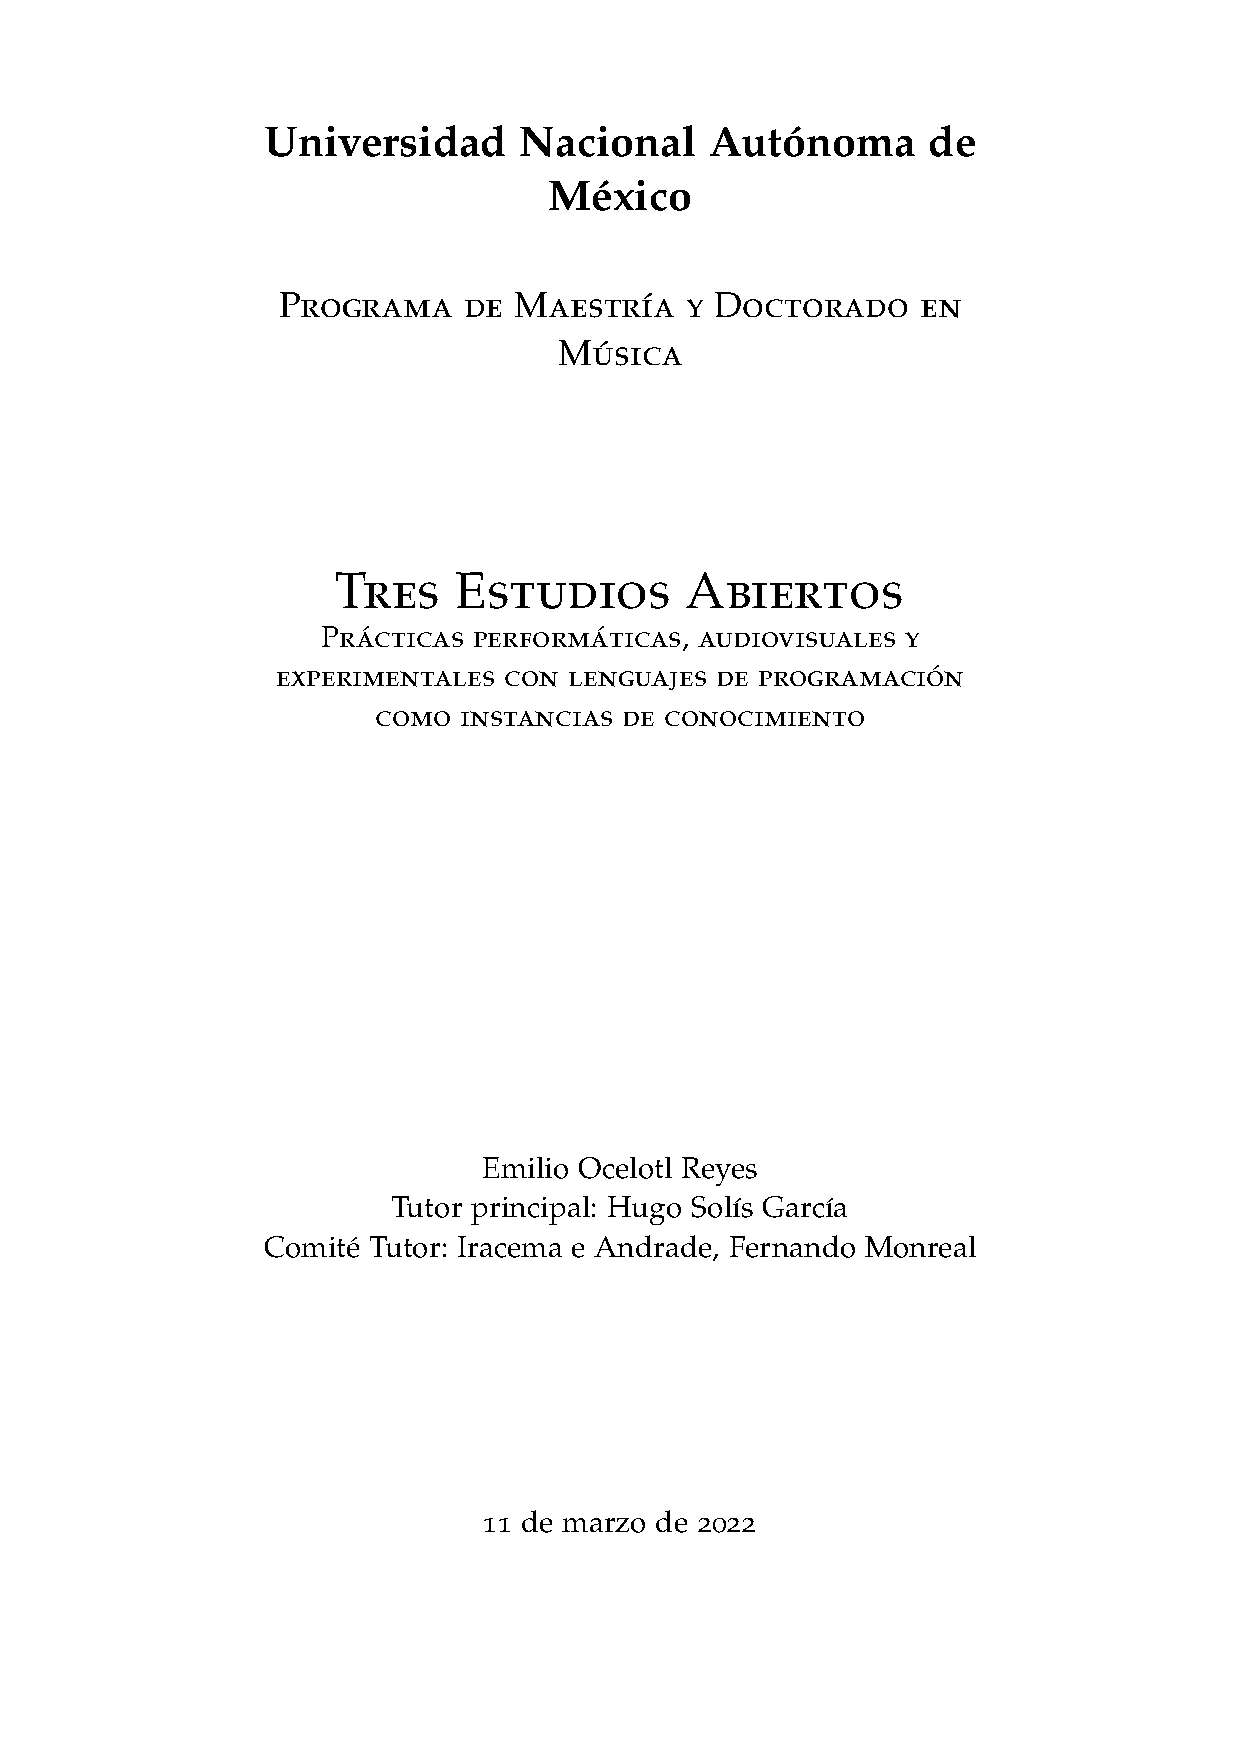
\includepdf{../portada/portada.pdf}

\tableofcontents
\listoffigures


%%----------------------------

% La propuesta es resumuir lo más posible esto
% Puntos de partida

%-----------------------------------------------

\chapter{Introducción}

%Descripción muy breve del proyecto 
%Motivación, algo breve.

La presente investigación es un bucle de investigación creación que estudia algunas prácticas performáticas, audiovisuales y experimentales con lenguajes de programación como instancias de conocimiento. De manera particular, señala un giro hacia las implicaciones de la interpretación audiovisual y la producción artística de obras para la web.

La estructura del documento es modular, cada subsección puede funcionar de manera independiente y puede ser leída como un artículo por sí mismo. La suma de estos módulos componen una investigación que puede leerse en lo general y en lo particular. 

A continuación, se esclarecen algunos puntos necesarios para la lectura de este documento. 

% La estructura y el resultado final del texto están pensados para la web,

\section{Contexto de escritura} % declaratoria de principios ? 

El contexto de escritura de este proyecto está marcado por una primera intención de desbordar laa investigación hacia la práctica de la música por computadora y la exploración con sonido. La generación de gráficos por computadora ha sido una extensión de esta exploración. Para el proyecto actual, representa un giro de acomplamiento que permite ampliar el rango práctico y reflexivo.

A manera de agente externo, la pandemia de COVID-19 ha marcado la vuelta definitiva de este proyecto hacia el navegador. Las experiencias particulares hacen patente las consecuencias que esto ha tenido para la investigación y la práctica artística. En relación a las preocupaciones centrales de esta investigación, el encierro y las posibilidades de la interconexión por medio de la web trajeron de vuelta la discusión sobre la presencia y la colaboración/interpretación/composición. 

\section{Obras}

El proyecto está vinculado por la realización tecnológica y práctica de piezas para el navegador que son objeto de la investigación. Las piezas son: anti, caso2 y caso3.

Estas piezas orbitan distintos lenguajes de programación y plataformas para la transformación de señales de audio y video y \gls{renderizacion} de gráficos tridimensionales. El centro de esta orbitación es \Gls{javascript}. 

\section{Software libre y de código abierto}

La perspectiva del \gls{softwarelibre} como un motivo para la investigación y práctica artística. De igual manera al código creativo, es importante señalar las implicaciones cercanas pero en algunos momentos contradictorias como el código abierto. Finalmente, establecer una crítica a la perspectiva redentora del software libre que contextualice el uso de la computadora como una interlocutora socialmente constituída por el trabajo de personas involucradas con la programación y la reflexión imbricada con el software.

% Perspectiva práctica. Aquí puedo hablar de lo que escribe JD y tomar el caso de Roberto

De manera particular, entendemos que las implicaciones del software libre y de código abierto tienen repercusiones en los resultados sonoros y visuales y especialmente, en las formas de organización social, económica y social de las personas que se involucran con lo que García llama sistemas de producción musical y que define como:

\begin{quote}

  ``un sistema de producción musical cuyos productos surgen de la interacción de personas que colaboran de manera distribuida, con herramientas, modos de operación y circuitos de distribución que funcionan bajo un principio generalizado de compartición y circulación libre de la cultura.''\citep[p.~65]{jorgeDavid2021}

\end{quote}

Este proyecto parte de motivaciones que expresan formas de practicar e investigar con y sobre tecnología. Algunas de las metodologías de trabajo que parten del hacer pero que desde nuestra perspectiva, se pueden extender al pensamiento y a la reflexión, están presentes en formas de trabajo como DIY o DIWO. Del giro y la problematización de estas herramientas en términos del trabajo en contextos colaborativos situados en latinoamérica retomamos perspectivas de trabajo como la que plantea y problematiza un espacio como Platohedro:

\begin{quote}

  ``El buen vivir sumak kawsay, demanda, en esta globalidad de conocimiento, de un sumak yachay, un buen conocer, de los saberes (nuevos y viejos). Es por tanto necesario desarrollar el buen conocer, aquel que beneficia a todos, que crea un entorno rico y fértil para la vida cultural, social, económica, política. En definitiva, crear una matriz productiva basada en conocimiento común y abierto''\citep[p.~31]{platohedro}

\end{quote}

% Por acá también podría ir algo referente a la decolonialidad 

La extensión de la cultura libre a otros ámbitos como a investigación artística o a la producción musical es uno de los puntos de partida de esta investigación. 

\section{Lenguajes de programación e investigación} % Podría ir en sobre este documento ? 

Partimos de la problematización de la práctica de la programación desde los estudios del software y tomamos la perspectiva de Winnie Soon y Geoff Cox para hablar de la programación como práctica:

\begin{quote}

``Consideramos la programación como una práctica cultural dinámica y un fenómeno, una forma de estar y hacer en el mundo y un medio para entender algunos de los complejos procedimientos que sustentan y constituyen nuestras realidades vividas, y para actuar sobre esas realidades'' \citep[p.~14]{aestheticProgramming}
  
\end{quote}

% Qué papel tienen las "ciencias del espíritu" de cara a la investigación artística que se centra en un tivo de investigación de las "ciencias exactas / naturales" ? 

Es por esto que retomamos algunas ideas de las ciencias sociales y de la observación participante. Como desplazar el centro de la investigación al sonido, la imagen o su integración como objetos de conocimiento por sí mismos. En este sentido, la investigación busca adentrarse en el código como una tecnología que permite establecer un tipo de relación entre los agentes involucrados. El caso de \cite{diProspero} ilustra el interés por vincular una práctica técnica con procesos sociales: ``La sociabilización en la actividad del live coding, se constituye, como veremos, en consonancia con la técnica, por lo cual se hace necesario un análisis que dé cuenta de la relación de los sujetos de estudio con la tecnología.''\citep[p.~48]{diProspero} Si los actores humanos son los sujetos de estudio de una investigación que se centra en tecnología y partiendo del marco Latouriano ¿Será posible plantear a la tecnología como la instancia del pensamimento de otros sujetos de estudio? ¿Cuáles serían las diferencias de estas instancias con respecto a la tecnología que no necesariamente se adscribe a un paradigma creativo o de práctica artística?

La problematización del marco de investigación investigación como algo presente en el proceso de escritura, como un objetivo secundario que pone en contradicción al investigador inmerso en una actividad práctica. El rodeo como un camino necesario para encontrar rutas no convencionales.

La ejecución y existencia de estas piezas supone un ecosistema de pensamientos prácticas y de otras piezas cercanas en términos tecnológicos y artísticos. La observación de estas piezas en contexto nos permitirá considerarlas como instancias de conocimiento que permitan a su vez, observar al paradigma de los lenguajes de programación como tecnología. De esta manera podemos contemplar las agencias que estas instancias por sí mismas tienen y que se les imputan en términos de relaciones políticas, sociales y económicas.

Este documento dialoga con perspectivas y prácticas que involucran lenguajes de programación. Codificación creativa ( Creative Coding ) y el término educativo \gls{STEAM} es una de ellas. En este sentido, la perspectiva educativa juega un papel importante como una extensión del paradigma que describimos. La presente investigación coincide con la aproximación artística y las observaciones críticas planteadas por Winnie Soon y Shelly Knotts con respecto a la programación:

\begin{quote}
  ``Esta aproximación estética no solamente incluye una introducción a la programación de manera práctica y creativa, sino también el cultivo de un espacio abierto donde sea posible discutir y reflexionar sobre la cultura computacional.''\citep[p.~87]{soonKnotts}

\end{quote}
  

Escalas de tiempo y la posibilidad de acercar/alejar la perspectiva y el contexto de lo que se investiga. La metáfora como una posibilidad para establecer trazos de conceptos entre hilos. 

% http://webtypography.net/

% Distribuited web of care y Taeyoon Choi 

\section{Versiones y repositorios}

El uso de \gls{git} como una herramienta para la escritura y el control de versiones, no solamente de código sino también de la parte escrita de la investigación. La investigación abierta. Crítica a estas plataformas y qué posibilidades existen de preservación de este documento en el contexto de tecnologías como la \emph{cadena de bloques} (blockchain) y \emph{wayback machine}. 

Dos referencias que establecen las posibilidades del trabajo con tecnología y escritura a partir del trabajo colaborativo y distribuido: Artículo de PiranhaLab y el artículo de PullPush. 

\chapter{Antecedentes}

% este apartado podría tener un orden: de lo más lejano a lo más cercano

% Aquí pienso colocar los antecedentes del proyecto.
% Me pregunto sobre la pertinencia de escribir una especie de estado del arte.
% Había pensado hablar de algunos proyectos cercanos que influyen en el proyecto
% Esto aparece ligeramente enunciado en el artículo de Panorama y en el texto que preparé para el coloquio
% Podría hacer un seguimiento al trabajo que hacen personas cercanas
% Incluso aquí podrían ir los primeros ejercicios en la web 
% Me imagino que aquí podrían aparecer algunos registros anectóticos 

Los antecedentes de esta investigación aluden a una trayectoria que va de la transición de la escritura de software para la realización de sistemas interactivos a la escritura de módulos de software audiovisuales. Estas experiencias toman como premisas la optimización y la ligereza de hardware (por ejemplo, con el uso de computadoras de placa reducida como Raspberry Pi o Jetson Nano ) y la elaboración sistemas ligeros, accesibles y portables para la síntesis y renderización audiovisual en el navegador.

A la par de la práctica artística con tecnología, los elementos precedentes de esta investigación se han conducido hacia la problematización del software como una instancia tanto de conocimiento como de ideas que conforman un paradigma que atraviesa todo el entramado de personas, investigaciones, escritos y obras involucrado con esta actividad. Estas reflexiones han tenido eco en el campo de investigación denominado estudios del software.

Los antecedentes a continuación descritos no necesariamente tienen un orden cronológico o de importancia. En todo caso es un compendio de perspectivas, plataformas, obras y realizaciones prácticas que desde la perspectiva de quien suscribe este texto, son relevantes de enunciar para captar las incidencias en los casos de investigación. 

%\section{Trilogía de Investigación}

%\textit{Tres Estudios Abiertos} forma parte de una trilogía de investigación. 

%\subsection{Objeto, Paisaje y Efecto}

%La primera parte fue Objeto, Paisaje y Efecto \citep{ocelotlLic}, un proyecto de investigación que abordó las nociones de objeto sonoro \citep{schaeffer}, paisaje sonoro\citep{schafer1} y efecto sonoro \citep{augoyard} para considerar a la escucha como un recurso para la investigación sociológica en música y para la investigación social desde el sonido.

%\subsection{Cuidado con la Brecha}

%Un segundo punto de investigación involucró un proceso de investigación-producción artística \citep{ocelotlMas}. La realización de este proyecto fue un prototipo tecnológico y partió de objetivos que inicialmente estaban propuestos como secundarios pero que más tarde se revelaron como parte del núcleo en la investigación. Estos aspectos son: 1) el proceso de trabajo colaborativo y su implementación con herramientas como git, 2) la reflexión sobre la interacción entre audio e imagen en la composición musical electroacústica y 3) el uso de herramientas libres, personalizadas para la realización de prototipos audiovisuales y para el planteamiento de una observación crítica de procesos creativos donde investigador y artista son el mismo agente. La propuesta de los estudios del software fue incorporada en este momento de investigación. 

%\subsection{Tres Estudios Abiertos}

%Referencia recursiva a esta investigación para explicar la trilogía

% \section{Música por computadora y algorítmica} % Esto se podría contradecir con el capítulo de marcos, peinso que esto se podría ir de aqui igual que el apartado de live coding 

%\subsection{Documenta X} % Pendiente tal vez podría ir en las conclusiones o como una problemmatización een la parte de montaje de anti

%Conexiones y accesos en muestras que implican espacios físicos y digitales. 

%\subsection{Plataformas}


%A continuación, haremos un breve rastreo de ideas centrales en la escritura de software orientado a la creación musical. El objetivo de este apartado consiste en describir y detectar la presencia del concepto unidad generadora en diversos programas orientados a la generación musical, de entre los cuales está una de las librerías que la presente investigación implementa.

%El punto de partida de esta indagación es MUSIC N, proyecto de Max Mathews que sería el parteaguas del paradigma de la música por computadora. Uno de los primeros casos de esta instancia es el principio de programas como Max/MSP y PureData, proyectos representativos de la programación gráfica presente en flujos de trabajo gráfico actuales como TouchDesigner.

%Como una observación adicional, es importante detectar instancias de la programación gráfica y de las ideas principales de la música por computadora en plataformas con giros programáticos particulares. Tal es el caso de OpenMusic, que de manera específica está basado en Common Lisp.

%Desde la perspectiva de la programación escrita, destacamos el papel que ha tenido SuperCollider en la extensión del paradigma de la música por computadora en la actualidad. Señalamos la importancia de SuperCollider como el motor bajo el cual se pueden ejecutar entornos de programación al vuelo como Tidal Cycles o FoxDot. 

%Estuary es un caso adicional que permite establecer un puente entre Tidal Cycles como un entorno que ejecuta SuperCollider como motor de audio y el navegador como tecnología multiplataforma sin instalaciones. Esta plataforma utiliza secuenciadores basados en la sintaxis de Tidal Cycles pero a diferencia del entorno que se puede instalar de manera local en una computadora, Estuary utiliza al navegador como motor de audio. 

%Trazamos estas relaciones para establecer una relación continua y presente entre los entornos anteriormente descritos y una de las librerías utilizadas en los casos de estudio de esta investigación: Tone.js. En este sentido, consideramos importante la adscripción a los principios de la música por computadora para encontrar soluciones personalizadas para el navegador.

%\subsection{Jacktrip y la música conectada}

%Una parte de los antecdentes de este proyecto se vinculan con la actividad del colectivo RGGTRN\footnote{\url{https://rggtrn.github.io/}. Consultado el \today} y del LiveCodeNet Ensamble\footnote{\url{https://livecodenetensamble.wordpress.com/}. Consultado el \today}

%RGGTRN es un colectivo de música por computadora fundado por Luis N. Del Angel y Emilio Ocelotl. Posteriormente se unieron Marianne Teixido y Jessica A. Rodríguez. Como parte de un ejercicio lúdico y de reflexión, el colectivo explora la improvisación audiovisual realizada por medio de código de programación, con una relación al contexto Latinx de sus participantes.

% Tesis de Luis
% Bellacode
% Saborítmico
% Tesis de maestría de hernani
% Artículo de Hernani en algún lado
% Artículos de Jessica ? 

%raspis conectadas y jacktrip > el trabajo realizado por CCRMA y en general 

%La labor del colectivo Radiador

% La radio y la transmisión de sonido con Icecast 

%Sonobus y la resolución de problemas de streaming en tiempos de pandemia

%\subsection{Fluxus y openGL}

%Para el caso de la imagen, retomo la influencia que tiene en la comunidad de live coding y en mi experienciación del performance audiovisual con la computadora el papel que tuvo el desarrollo Fluxus\footnote{\url{https://gitlab.com/nebogeo/fluxus/}} de Dave Griffiths que se remonta al 2007. Una característica peculiar de este desarrollo es el uso de una sintaxis tipo LISP que recuerda a desarrollos musicales basados en este lenguaje de programación como OpenMusic. 

%Detrás de Fluxus también cabe destacar la importancia de sistemas de renderización de gráficos por computadora como OpenGL, que actualmente, son el punto de partida de software de alto nivel involucrado con este proyecto como OpenFrameworks y la variante para el navegador, webGL, que implementa la librería Three.js 

% Pregunta, esto no tendría que ir en otros momentos? Tal vez disperso o tal vez en la introducción 

%\section{Live Coding} % Pregunta: Este apartatdo no debería ir antes ? En momentos anteriores menciono la cuestión  

% Antecedentes más extensos

%Encuentro múltiples formas de abordar el tema. El live coding puede describirse en térrminos de unaa comunidad que realiza una práctica y que se enuncia como tal, como un sub-campo creativo que comparte elementos con otra expresiones como la música algorítmica y el arte generativo. Finalmente, el live coding podría acotarse a motivos de investigación académica e independiente y a la realización tecnlógica de interfaces de texto que corren sobre motores de audio y video.

%De estas múltiples formas de abordar el fenómeno y de acuerdo a los fines de esta investigación, nos preguntamos si el eje que las articula son discusiones sobre el lenguaje y la escritura. 

%\subsection{Primeras expresiones}

%Antecedentes del live coding: la escena mod.

%En el manifiesto del live coding se expresan pensamientos que hasta el momento, son vigentes. 

% PhD Thesis: Artist-Programmers and Programming Languages for the Arts - Alex McLean 
%Dentro de los antecedentes está la experiencia performática de escribir código al vuelo con fines creativos, audiovisuales y experimentales.

%Las primeras expresiones reflexivas y prácticas del live coding no solamente establecen puntos de partida performáticas, sino que al mismo tiempo aportan elementos para el diseño y análisis de sistemas basados en interfaces de código:

%\begin{quote}

%  ``Nuestro argumento nos lleva a través de capas de representación, comenzando con símbolos, luego palabras, lenguaje y notación, para considerar el papel que estas representaciones pueden jugar en la creatividad humana'' \citep[p.~3]{McLean2011}

%\end{quote}

%La noción de capas de representación permite analizar la complejidad del proceso artístico con código en términos de la relación entre humanos y los aspectos cognitivos, sociales y políticos que les atraviesan, y los no-humanos en lo que respecta a las posibilidades de conocimiento instanciado presentes en ellos. 

%Live coding desde cero y la improvisación. 

%\subsection{Nodos y circuitos}

%La práctica de la programación al vuelo, delimitada técnica, escénica, musical y visualmente se origina en Inglaterra. % cita

%Como lo describen \cite{villasenor} para los casos de Barcelona y Ciudad de México.\footnote{Un ejemplo reciente se encuentra en: \url{https://youtu.be/n5kwi4eRAE4}} 

%\subsection{Exploración visual}

%Exploración visual para la integración con el sonido.  

%\begin{figure}[tb]
%\centering 
%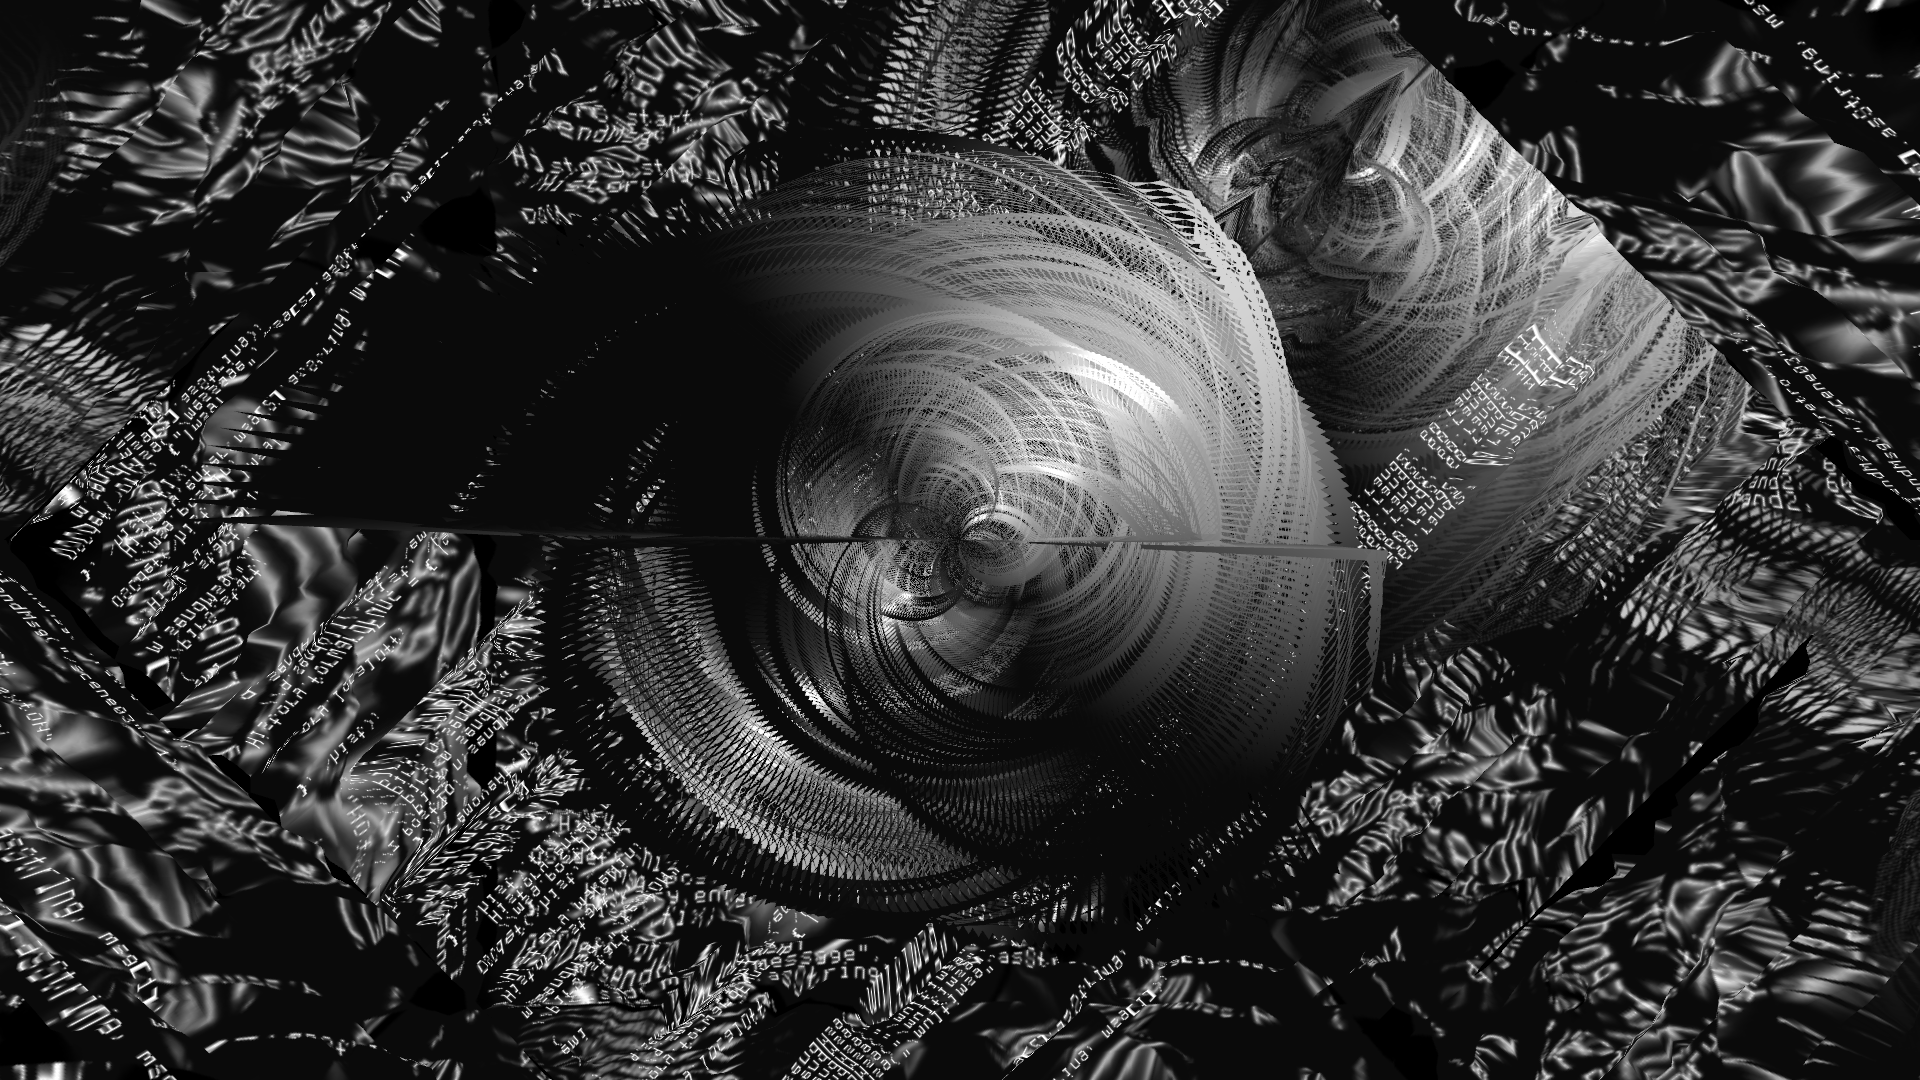
\includegraphics[width=\columnwidth]{../img/of13.png} 
%\caption[Openframeworks 1]{Captura de render realizado con OpenFrameworks} % The text in the square bracket is the caption for the list of figures while the text in the curly brackets is the figure caption
%\label{fig:gallery} 
%\end{figure}

%El campo del live coding tuvo un giro importante con la llegada de hydra de Olivia Jack. La rápida expansión de esta plataforma y la sintaxis que recuerda la conexión de flujos de energía similar a los sintetizadores analógicos favorecieron la producción de piezas e interpretaciones enfocadas en la imagen y en algunos otros casos a la par del audio. La importancia de esta plataforma ha delimitado una estética  basada en  la transformación de píxeles, de formas y de transformaciones basadas en funciones matemáticas.

%En palabras de Olivia Jack, los procesos que realiza la computadora hay un eje de profundidad, en términos del despliegue gráfico físico de la computadora de espacios bi o tridimensionales, el resultado es bidimensional.

%La lógica de Hydra es modular, esto quiere decir que puede incorporarse como un componente adicional a proyectos que no necesariamente se centren en la producción visual con esta plataforma. Esta modularidad juega a favor de lenguajes de programación como Javascript. 

\section{Proyectos Colindantes}

Algunos proyectos cercanos tecnológica, conceptual y estéticamente a \emph{Tres Estudios Abiertos} son: 

\subsection{Nivel Bajo}

\begin{itemize}

\item Ruffbox\footnote{\url{https://github.com/the-drunk-coder/ruffbox}}
\item WebAssembly/Rust Tutorial\footnote{\url{https://www.toptal.com/webassembly/webassembly-rust-tutorial-web-audio}}
\item Flocking\footnote{\url{https://github.com/continuing-creativity/Flocking/}}
\end{itemize}

\subsection{Nivel Medio}

\begin{itemize}

\item supercollider.web\footnote{\url{https://github.com/khilnani/supercollider.web/}}
\item Web Audio API\footnote{\url{https://developer.mozilla.org/es/docs/Web/API/Web_Audio_API}}
\item Tone.js\footnote{\url{https://tonejs.github.io/}}
\item SuperCollider.js\footnote{\url{https://github.com/crucialfelix/supercolliderjs/}}
  
\end{itemize}

\subsection{Nivel Alto y Ecosistemas}

\subsubsection{Nivel Alto}

\begin{itemize}
\item Hydra\footnote{\url{https://github.com/ojack/hydra}}
\item Troop\footnote{\url{https://github.com/Qirky/Troop}}
\item flok\footnote{\url{https://github.com/munshkr/flok}}
\item tilt\footnote{\url{https://github.com/munshkr/tilt}}
\item LiveLab\footnote{\url{https://github.com/ojack/LiveLab}}
\item timeNot\footnote{\url{https://github.com/luisnavarrodelangel/seis8s}}
\item seis8s\footnote{\url{https://github.com/AFrancoB/timeNot}}
\item Camposonico\footnote{\url{https://github.com/diegovdc/camposonico}}
\item INSTRUMENT\footnote{\url{https://github.com/punksnotdev/INSTRUMENT}}
\end{itemize}


\subsubsection{Ecosistemas}

\begin{itemize}
\item Estuary\footnote{\url{https://github.com/dktr0/estuary}}
\item Sema-engine\footnote{\url{https://github.com/frantic0/sema-enginef}}
\end{itemize}

\section{Piezas y obras lejanas}

\subsection{Notas de Ausencia} % Cambiar la redacción para que no sea exactamente igual al artículo de panorama 

Notas de Ausencia de Marianne Teixido  es un ensayo generativo en la web. Utiliza texto-dato que por medio de la computadora como agente resignificante, deconstruye estructuras discursivas para resemantizar la narrativa sobre las desapariciones de mujeres en México y América Latina.

\begin{figure}[tb]
\centering 
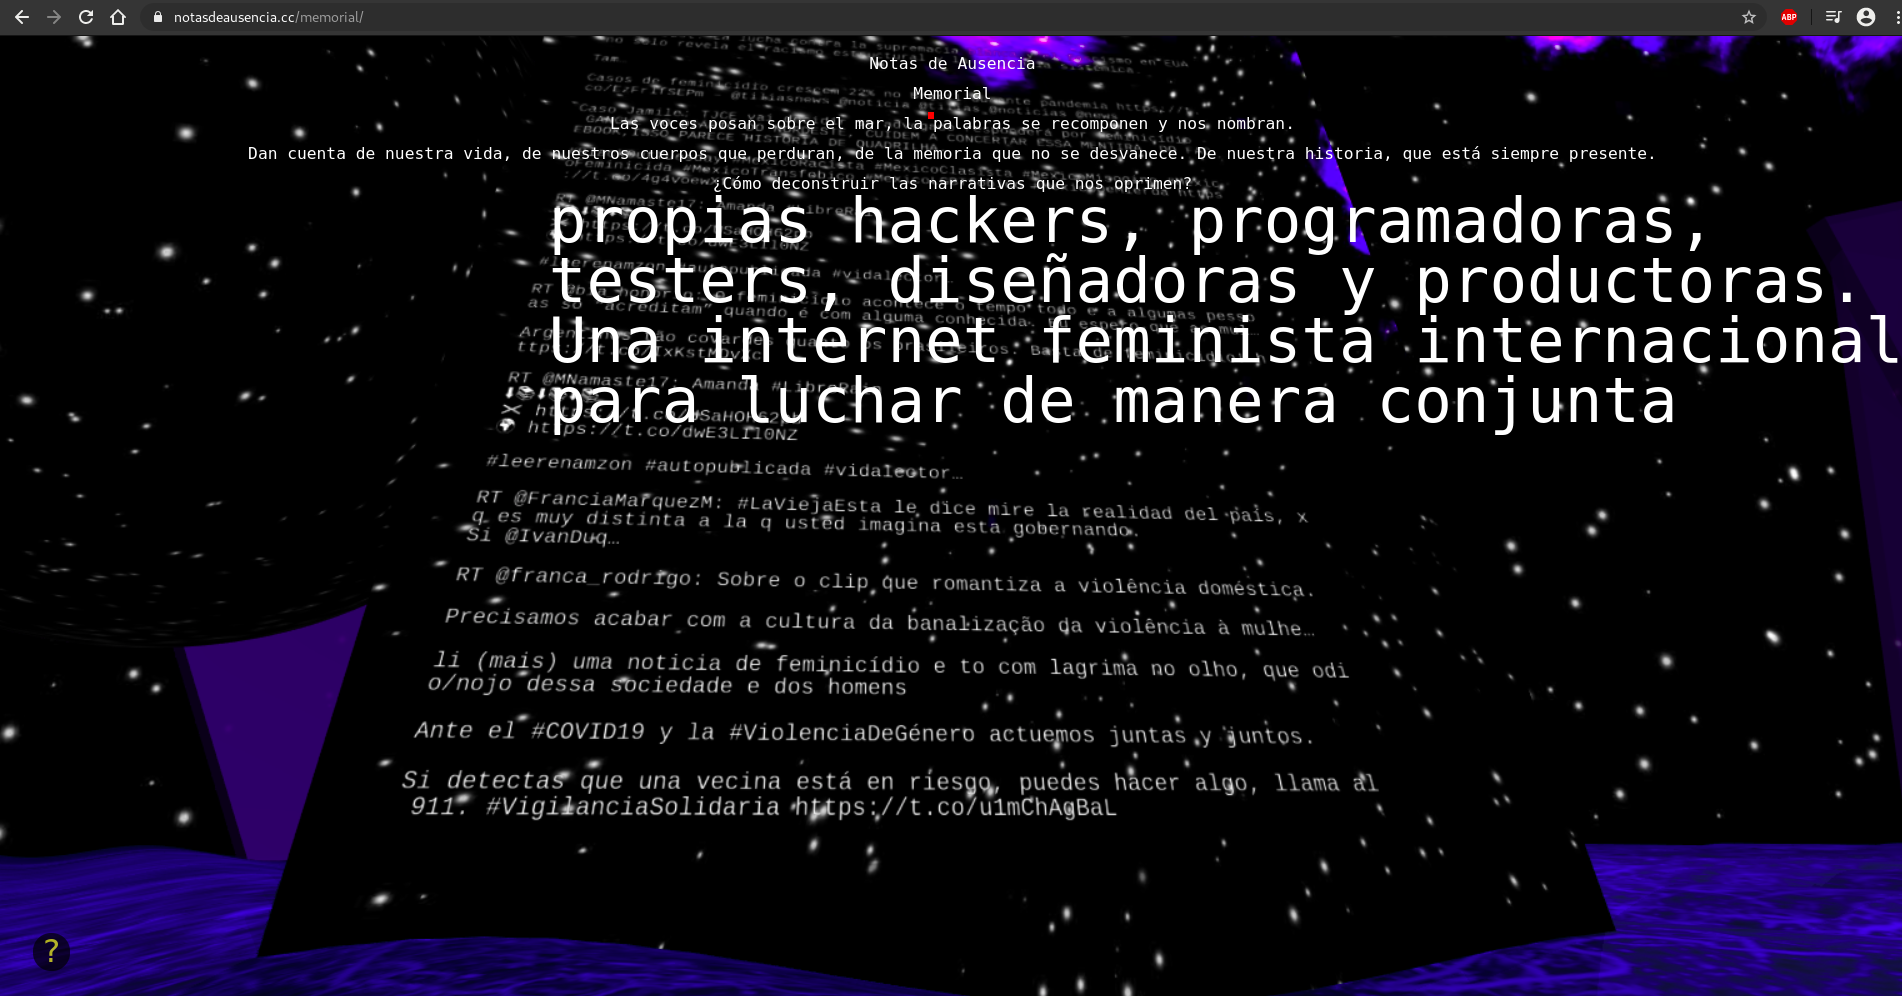
\includegraphics[width=\columnwidth]{../img/notas02.png} 
\caption[Notas de Ausencia - Marianne Teixido]{Captura de Notas de Ausencia de Marianne Teixido. Consultado el \today en: \url{https://github.com/MarianneTeixido/notasdeausencia}} % The text in the square bracket is the caption for the list of figures while the text in the curly brackets is the figure caption
\label{fig:gallery} 
\end{figure}

El tiempo y espacio virtual conforman una partitura para la memoria y la denuncia. La narrativa, semi-autónoma, argumenta a partir de textos tomados de tweets, poemarios, libros y artículos feministas que explican desde la teoría las desapariciones forzadas, el feminicidio y la violencia de género. Estos elementos están presentes como texto, imagen y sonido en un espacio tridimensional diseñado a manera de memorial.

La narrativa de la pieza está articulada mediante la intervención de dos bots que interactúan en Twitter. El primero realiza una búsqueda de tuits a partir de un filtro de palabras clave escritas como hashtags como: \#MéxicoFeminicida, \#MadresEnBúsqueda, \#ViolenciadeGenero, \#NiUnaMenos, entre otros.\footnote{Al momento de escritura, el bot se encuentra activo en la cuenta: \url{https://twitter.com/notasausencia} (Consultado el \today} Posteriormente, recomparte el tuit que contiene alguno de los hashtags de la base de datos previamente delimitada. El segundo bot retoma los textos de los tuits seleccionados y los remixea para generar un segundo texto automático por medio de cadenas de Markov.

Esta pieza se realizó en el contexto de la exhibición en línea Creaciones con Algoritmos: Visualización y Sonificación de Datos del Centro de Cultura Digital en abril de 2020. Su salida oficial se realizó en video sin embargo, el planeamiento original contempló la creación de un espacio virtual en la web que pudiera visualizar en tiempo real la información viva proveniente de los tweets.

Dos características definieron el diseño de la pieza: ubicación de la pieza en un espacio tridimensional y la interacción y visualización de la información proporcionada por los bots. Para la realización, el proyecto retomó módulos iniciales de Panorama y partió del uso de Three.js como un entorno de trabajo que pudiera conectar los dos momentos de la pieza antes descritos.

\subsection{Hydra, visuales y el navegador}

Uno de los referentes en términos de live coding con resultados visuales es la obra de Olivia Jack. La realización de éstas va de la mano con el software desarrollado por ella misma: Hydra. El proyecto está alojado en la web y la descripción se define como: ``[U]na plataforma para live codear visuales, en la que cada ventana del browser puede ser usado como un nodo de un sintetizador de video, modular y distribuido'' \footnote{Consultado el \today en: \url{hydra.ojack.xyz}}

Hydra es un proyecto abierto y libre, lo cual permite que una comunidad de usuarios se involucren en el uso, mantenimiento y expansión del repositorio. Algunos proyectos que utilizan directa o indirectamente hydra.

Destacamos del proyecto la sintaxis personalizada que permite controlar el resultado visual a partir de funciones y parámetros. Estas funciones pueden anidarse y concatenarse, lo cual da como resultado una serie de instrucciones aglutinadas y encadenadas. Este continuo coincide con la analogía del patcheo de los sintetizadores modulares de audio y video. 

\subsection{The Stage is (A)Live}

The stage is (a)Live\footnote{\url{https://www.geometries.xyz/theStageIsAlive/}} - Johana Chicau y Renick Bell


%\section{Piezas y obras cercanas} % Pendiente, igual y no hay tantas cosas 

%\subsection{Pumpumyatchkan}

%\begin{figure}[tb]
%\centering 
%\includegraphics[width=\columnwidth]{../img/pumpum.JPG} 
%\caption[Concierto PUMPUM]{Presentación en el festival PUMPUM} % The text in the square bracket is the caption for the list of figures while the text in the curly brackets is the figure caption
%\label{fig:gallery} 
%\end{figure}

%\subsection{Concierto de clausura} % Este si podría ser relevante 

%Concierto virtual realizado en el marco del coloquio de alumnas del Programa de Posgrado en Música de la UNAM

%\begin{figure}[tb]
%\centering 
%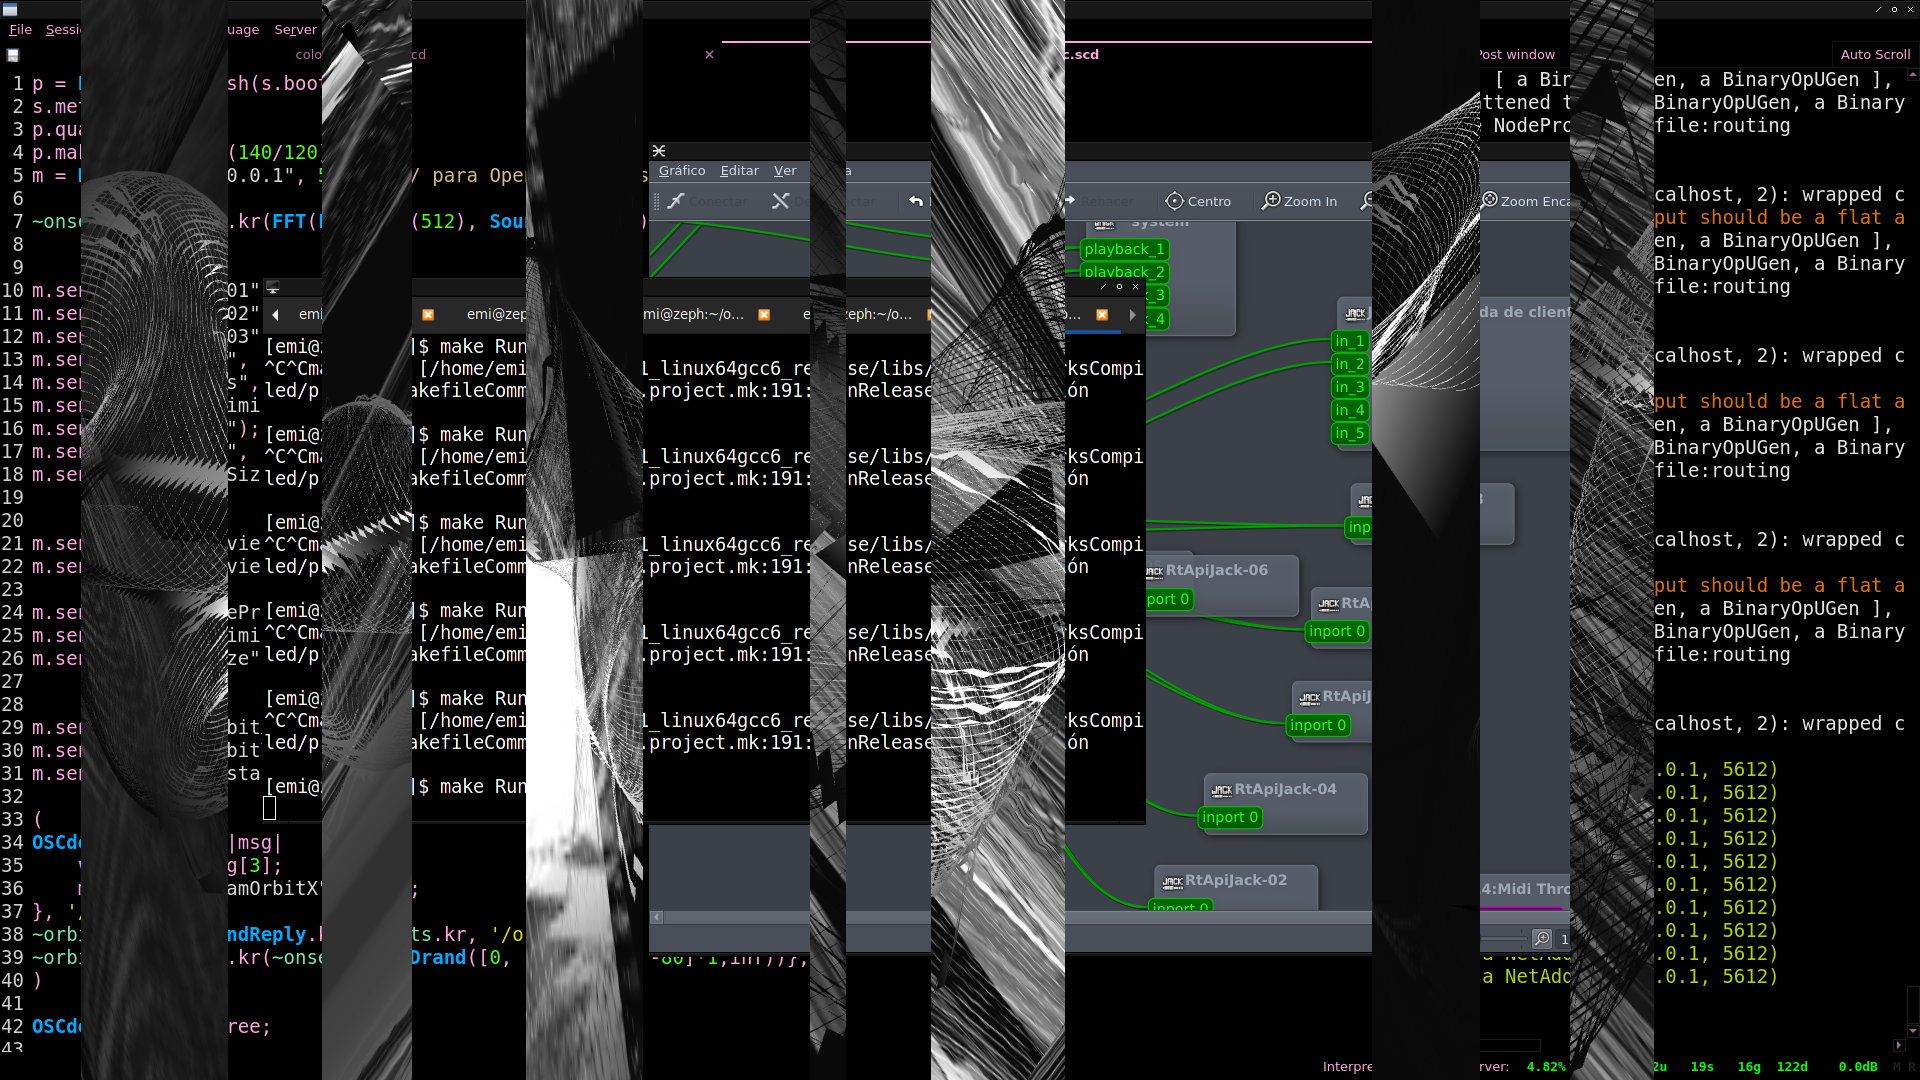
\includegraphics[width=\columnwidth]{../img/col2.png} 
%\caption[Concierto coloquio]{Captura del concierto del Coloquio de alumnas \url{https://youtu.be/HwBTRQKr9Ps}.} % The text in the square bracket is the caption for the list of figures while the text in the curly brackets is the figure caption
%\label{fig:gallery} 
%\end{figure}

\section{PiranhaLab}

Otro antecedente de este proyecto es la práctica y reflexión planteada en colectivo por\textit{PiranhaLab}\footnote{``PiranhaLab es un laboratorio interdisciplinario que trabaja en las tripas del software''. \url{https://piranhalab.github.io/} (Consultado el \today)}.

\subsection{Escritura de y con software}

\subsection{Ciclo de Talleres}

El ciclo de talleres realizado en el Centro de Cultura Digital (CCD) en coparticipación con el Laboratorio de Tecnologías Libres\footnote{Actualmente Laboratorio de Tecnologías Compartidas} permitió plantear dos conclusiones que se heredan a \textit{Tres Estudios Abiertos}: La difuminación de la distinción usuario/desarrollador como una motivación para la escritura de software y la procuración de diversidad en la escritura de software en América Latina.

\begin{figure}[tb]
\centering 
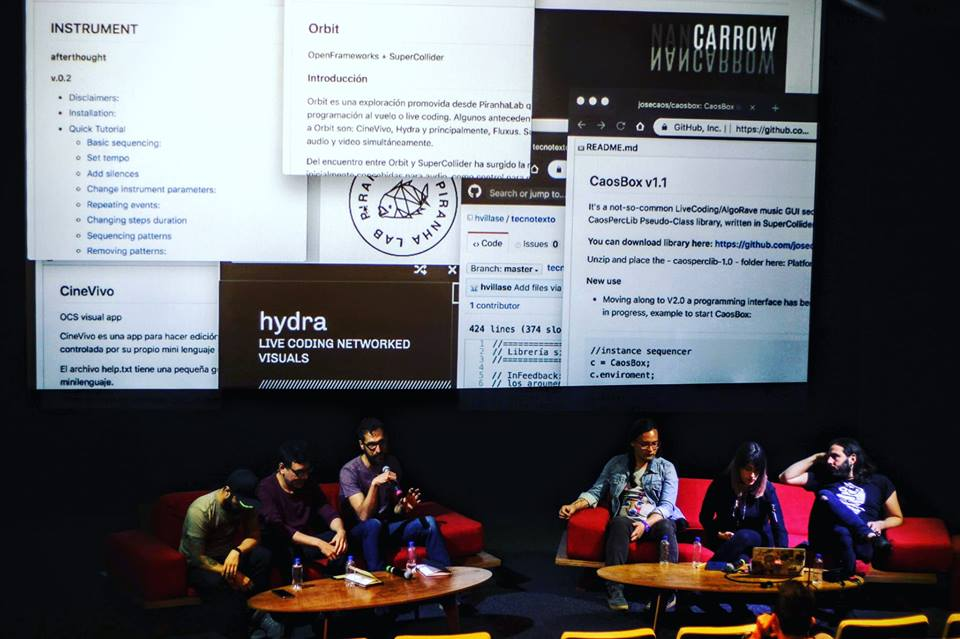
\includegraphics[width=\columnwidth]{../img/conversatorio.jpg} 
\caption[Conversatorio CCD]{Conversatorio organizado por PiranhaLab y el Laboratorio de Tecnologías Compartidas en el CCD. 2019.} % The text in the square bracket is the caption for the list of figures while the text in the curly brackets is the figure caption
\label{fig:gallery} 
\end{figure}

\subsection{EDGES 2020}

La escritura de espacios para el ciclo de conciertos EDGES 2020 realizado por el Taller de Imágenes en Movimiento del Centro Multimedia (CMM) permitió la exploración de entornos tridimensionales inmersivos en el navegador en el contexto del encierro causado por la pandemia de COVID-19. Técnica y conceptualmente la escritura de estos espacios digitales influye en el presente proyecto. El artículo \textit{Panorama} \citep{panoramaArticulo} hace referencia de manera extensa al ecosistema de espacios y propuestas que también inciden en \textit{Tres Estudios Abiertos}.

% Esto se articula con las actividades colectivas de la sección casos 

Espacios inmersivos que estuvieron activos de manera simultánea. 

\section{Seminario Permanente de Tecnología Musical} 
% \printendnotes

%%% Esto podría no ser necesariamente un capítulo sino una serie de apuntes distribuidos en la tesis. Esto para ser congruente con la idea del bucle investigación-creación en música con tecnología 

\chapter{Perspectivas de investigación}

\section{Giro de los nuevos medios}

\textit{Tres Estudios Abiertos} retoma esta incorporación, parte del giro de los nuevos medios y de los estudios del software \citep{manovichlanguage}.

\section{Estudios del software y código}

Como una extensión del punto de partida, la investigación se adscribe a la escritura con y sobre software \citep{aestheticProgramming}.

\section{Programación y práctica artística}

Atiende al papel que juega la experiencia subjetiva y las implicaciones políticas y sociales en la programación que se extiende y se posibilita por las prácticas artísticas \citep{speakingCode}. 

Investigaciones cercanas que resuelven problemas similares (hasta el momento):

% Aquí puede ir el apartado de el código como partitura y como ejecución y la relación con austin 


\section{El código como agente y como prótesis}

Carolina di Prospero y Bruno Latour como referencias para explicar esta relación. 

% Tesis doctoral de Roberto Cabezas. 

% La arquitectura propuesta en las siguientes líneas (como bien se ha mencionado anteriormente) no tiene el enfoque de la máquina como entidad creativa autónoma, sino más bien como herramienta de expansión cognitiva, en torno a las posibilidades del dominio epistémico y en función de las imágenes culturales osociales que intervienen en los procesos creativos del ser humano

% La computadora o la máquina como una prótesis y no como un agente autónomo. Es posible resolver esta distinción a partir de la idea del trabajo muerto ? 

% El uso del aprendizaje automático tiene una meta concreta, la cual es la expansión del dominio epistémico para la construcción de nuevos ejemplos en el conjunto de datos híbridos y la transformación del espacio conceptual.

% Esta discusión puede ir en el apartado de anti. La pregunta es si hay una sola meta en el aprendizaje automático 

% Los sistemas computacionales híbridos son entonces una propuesta recursiva computacional, en la que la simbiosis ocurre cuando consideramos al ser humano un organismo capaz de realizar computación, en donde el tiempo de computación puede ser interrumpido para valorar mediante la percepción la inclusión de nuevos datos al espacio conceptual. Al final los humanos son los que encuentran la semántica en la salida de las máquinas.

% Interesante lo del tiempo, ahí podemos agregar la cuestión de las magnitudes de tiempo y espacio

% En general el principal beneficio del desarrollo de técnicas y nuevas arquitecturas de aprendizaje profundo se ha visto en áreas de visión por computadora, salud o biología sintética, pero el arte y el diseño también se han beneficiado de estos avances, puesto que existen laboratorios de investigación totalmente dedicados a explorar —en específico— el aprendizaje profundo con fines creativos o, en su defecto, cómo utilizar la investigación artística para encontrar nuevas aplicaciones para estas técnicas de computación en la sociedad actual.

% En algún momento aparece pero no está citado aqui: el papel que tiene esta tecnología para la industria y en qué momentos industria y creación parecen lo mismo. Anti 

% El uso de las GAN’s para el diseño de sistemas computacionales, puede ser el detonante para el cambio de paradigma hacia los roles de las máquinas en procesos creativos. El proyecto anterior, aunque sus resultados sonverdaderamente impresionantes, mantiene el paradigma convencional de investigación: la máquina como entidad autónoma de creación, lo que de algunamanera no fomenta el avance del ser humano como un creador más completo o expandido.

% El papel de la previsualización

% La implementación de la GAN utilizada en CLUSTER se realizó con la librería Keras como interfaz simplificada de Tensorflow y, la arquitectura general fue tomada de (Mao, Li, Xie, Lau, Wang, & Smolley, 2017) con las llamadas Redes Adversarias Generativas de Mínimos Cuadrados (LSGAN’s).

% \printendnotes


% Primer capítulo 

% \chapter{Casos}

En este apartado describo los casos específicos

Ejes: Las escrituras, sonido e imagen como formas de conocimiento y lenguajes de programación y estructura

Diferentes capas que pueden ser artículadas por medio del sonido. Los antecedentes y el contexto podrían ser la dimensión temporal que rebasa mi obra. 

¿ Más casos particulares tipo obra ? 

% \section{Ecosistema}

% Articulación con una propuesta de investigación que quedo deshechada. ¿Es posible potenciar los proyectos en un contexto social, es decir, en una dimensión que rebasa la propia obra (y por lo tanto el individuo) ? 

Ecosistema como una forma de nombrar al entramado de Nodos y Trayectos. 

¿En qué contexto se inserta mi proyecto ? Impulso de desarrollos o DWO

Un referente que no necesariamente sea una pieza artística pero que genere condiciones para la práctica. 

%  \section{Interfaz}

La interfaz como una posibilidad de la escritura de código y del proyecto de investigación 

% \subfile{sec/anti/anti}

% \chapter{Efectos de conocimiento}

Este capítulo contendrá la perspectiva de investigación: puntos de partida teóricos y metodológicos para analizar procesos artísticos instanciados en lenguajes de programación. 


% \chapter{Caso 1: THREE.studies}

 THREE.studies es una pieza para el navegador que aprovecha las posibilildades del intercambio de flujos de audio y video. 

\section{Delimitacicón y contexto}

THREE.studies fue realizada en conjunto con Iracema de Andrade y con el apoyo técnico del colectivo PiranhaLab y fue apoyada por el programa Resiliencia Sonora de Música UNAM. El proyecto surge como un primer acercamiento a la realización de piezas que de alguna forma, puedan interactuar con intérpretes de forma remota. El contexto pandémico en este caso fue un detonador de una serie de pruebas realizadas para producir una pieza en tiempo real utilizando canales de comunicación en la web. 

SEALI 

\section{Versiones anteriores} 

La pieza fue estrenada en el marco del festival BEAST FEaST, organiado por la universidad de Birhminham. Cabe destascar que esta versión nunca tuvo una versión presencial. 

\begin{figure}[tb]
\centering
\subfloat[Primera Versión de THREE.studies]{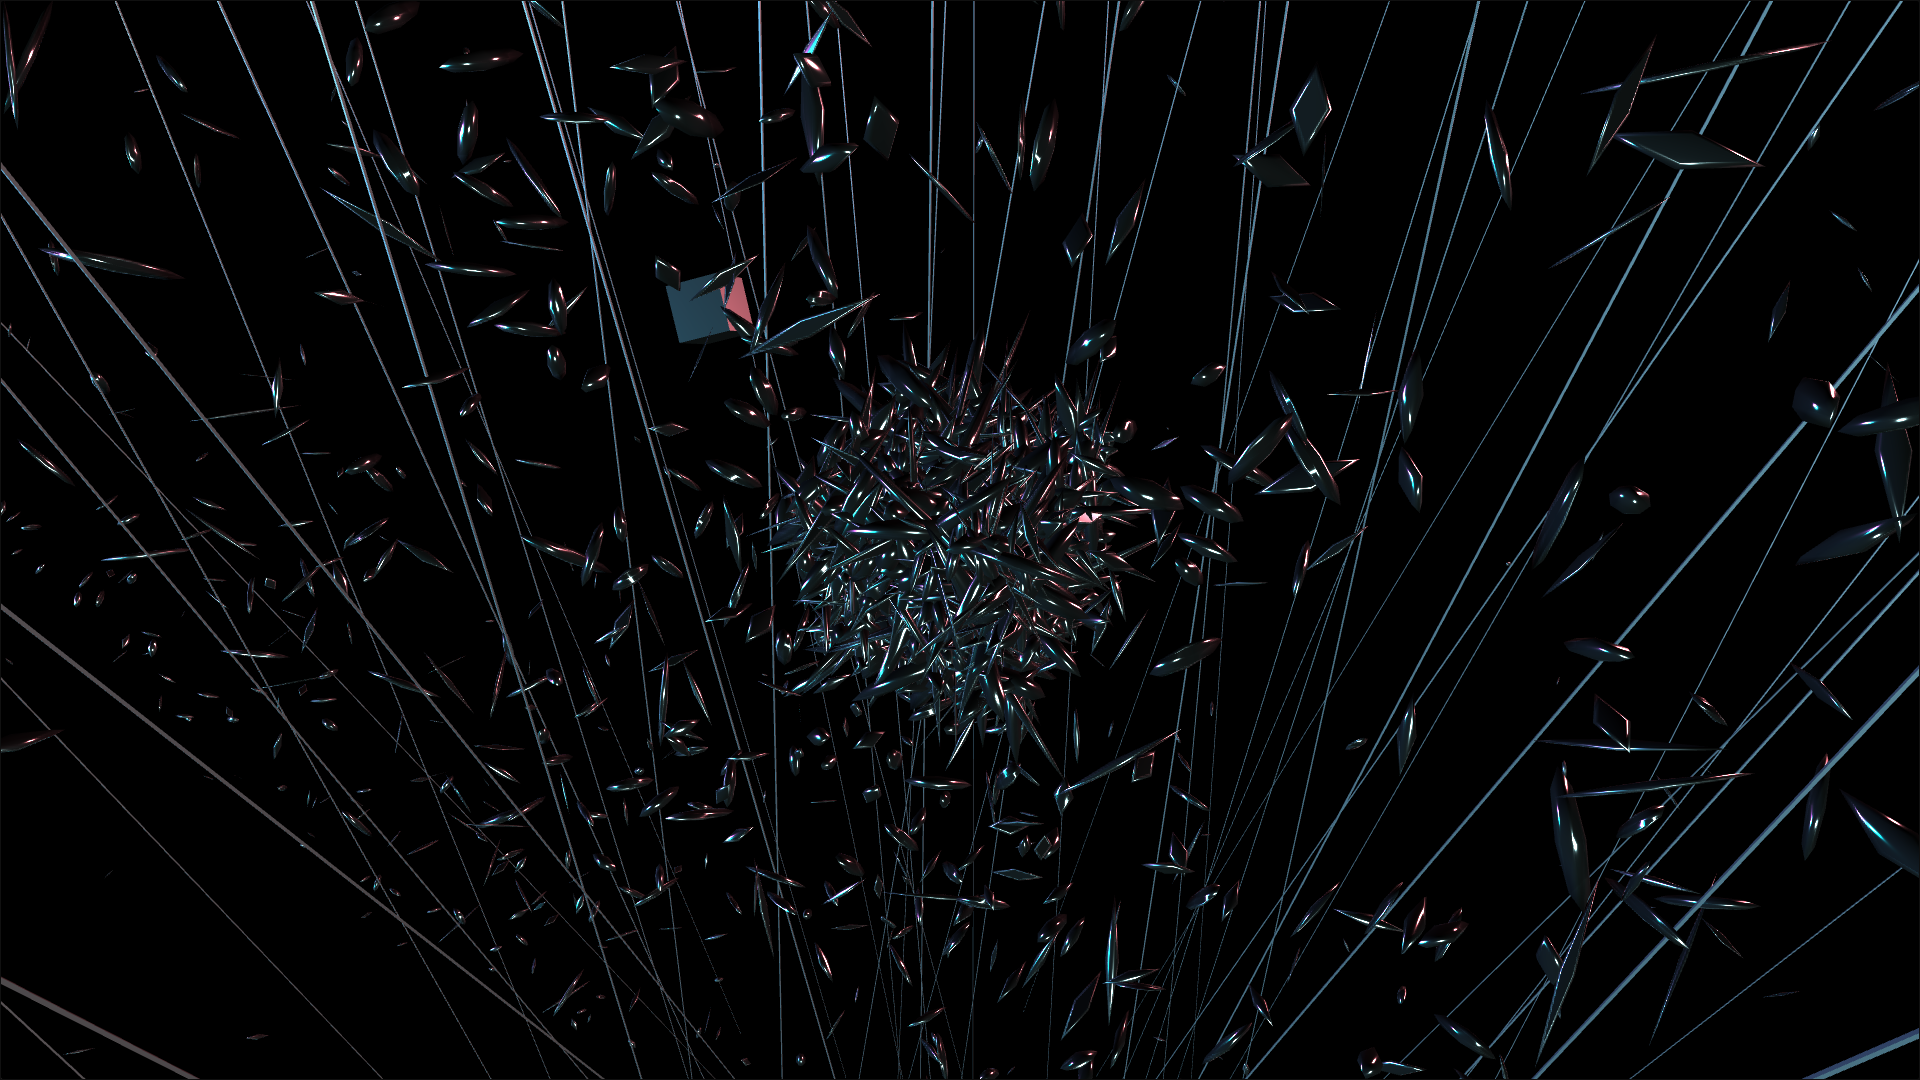
\includegraphics[width=\columnwidth]{../img/beast.png}} \quad
\subfloat[Segunda versión de THREE.studies]{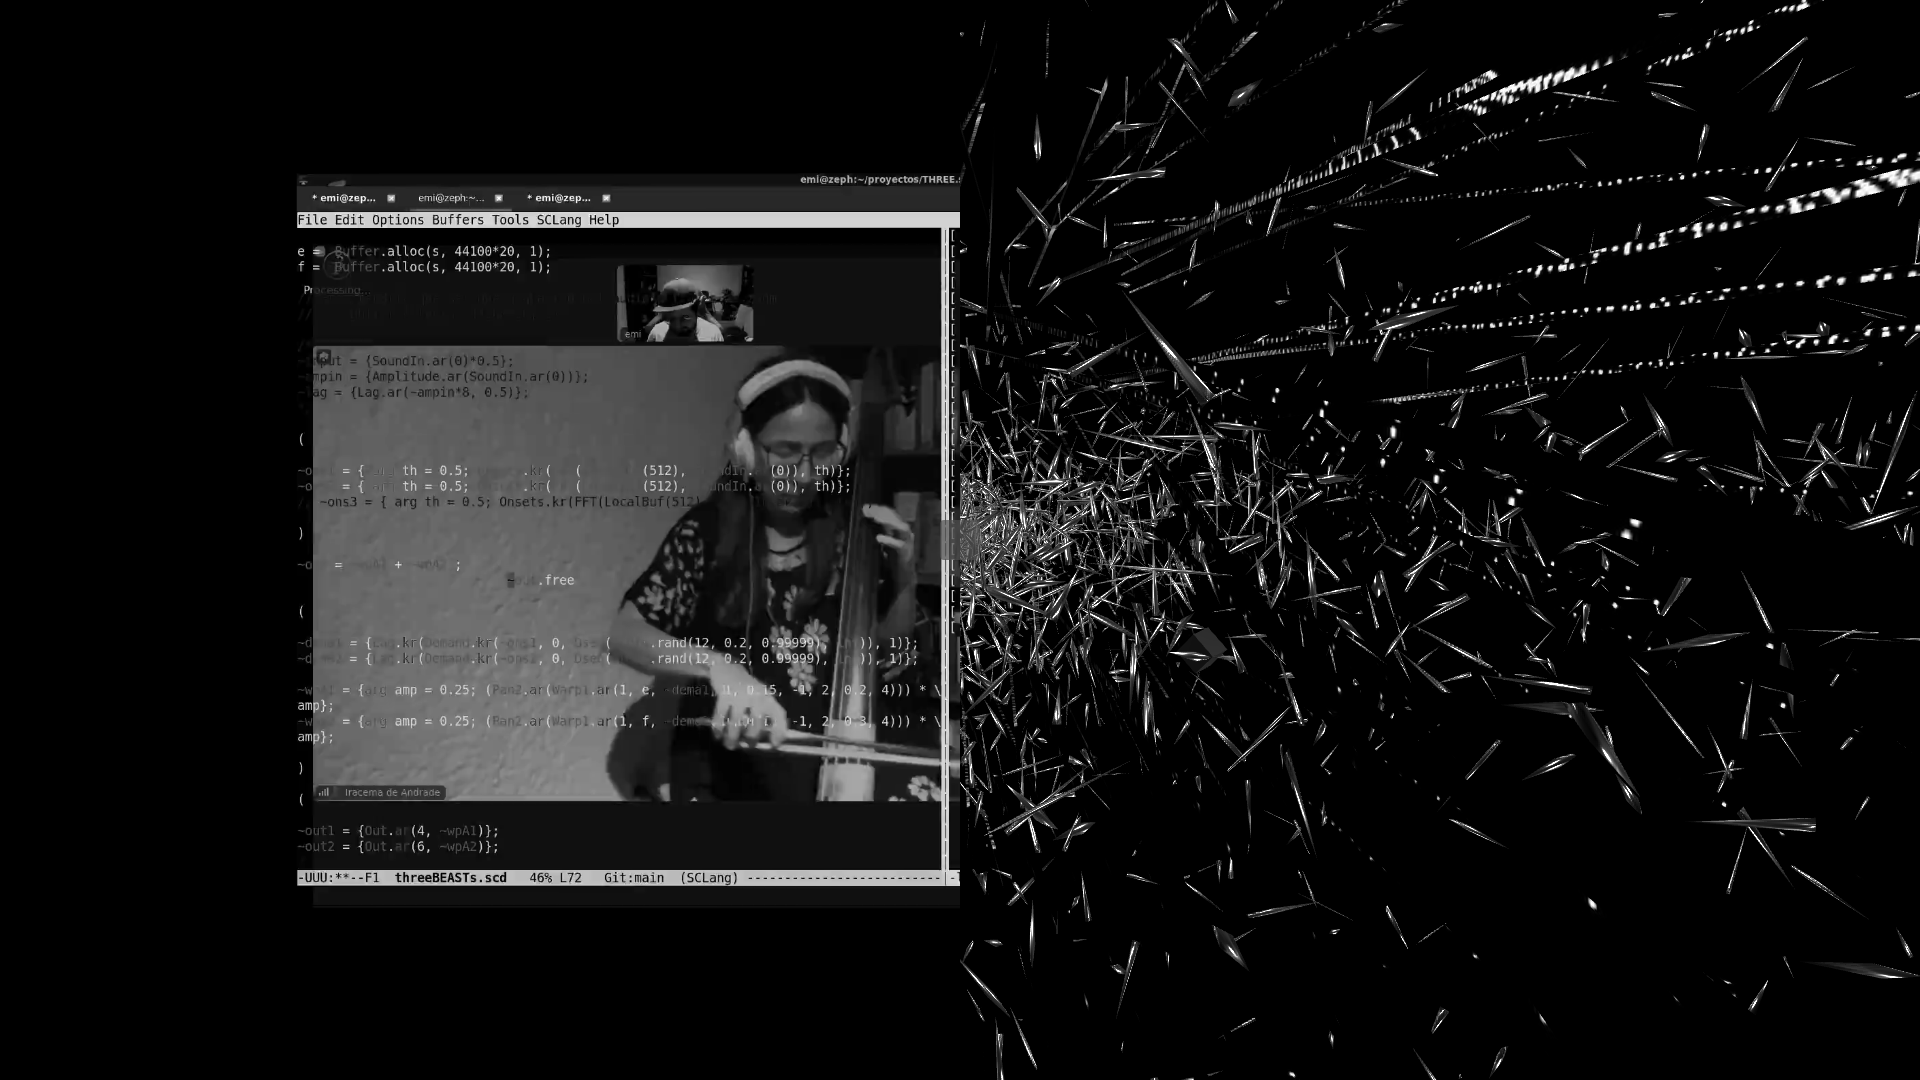
\includegraphics[width=\columnwidth]{../img/threeNw.png}\label{fig:ipsum}} 
\caption[Versiones de THREE.studies]{Versiones de THREE.studies ordenadas cronológicamente} % The text in the square bracket is the caption for the list of figures while the text in the curly brackets is the figure caption
\label{fig:esempio}
\end{figure}

El proyecto se mantuvo en transformación. El video del proceso quedó registrado y fue posible utilizarlo para visualizarlo dentro del espacio virtual. 

\section{Version final}

El futuro podría implicar el uso de capturas tridimensionales de Iracema y reforzar el input de sonido a partir de la visualización de gestualidades fijadas en un objeto tridimensional. Una primera prueba del sistema basado en History podría implicar la reproducción del history como una pianola de código que pudiera imprimirse en el espacio virtual. En este sentido se podría prescindir de un video y dar cuenta del performance a partir de algunos efectos capturados del mismo: gestualidades en 3d, audio y código ejecutado en el tiempo. 

%\chapter{Caso 2: Anti}

% Este apartado puede convertirse en un artículo por sí mismo. Describirlo de una manera distinta al tipo contexto, planteamiento, proceso y resultados  

% \href{https://anti.ocelotl.cc}{\includegraphics[width=\textwidth]{img/anti01.png}} % Una imagen que también es hipervínculo 

\begin{figure}[tb]
\centering 
\includegraphics[width=\columnwidth]{../img/anti01.png} 
\caption[Captura de Anti]{Captura de anti y de la interfaz gráfica que utiliza de \url{https://anti.ocelotl.cc}.} % The text in the square bracket is the caption for the list of figures while the text in the curly brackets is the figure caption
\label{fig:gallery} 
\end{figure}

% Anti es una pieza que parte de la ofuscación para plantear una reflexión sobre la relación que existe entre usuarios y tecnología. Utiliza algunos módulos de \gls{aprendizajeautomatico} (machine learning) 

%\subsection{Contexto}

\iftoggle{tesis}
{La ofuscación puede definirse como el acto deliberado de encubrir el significado de una comunicación. Para el caso de la programación y apuntando ideas hacia los estudios del software, la presente investigación toma la noción de ofuscación de un conjunto de posibilidades para la escritura de software que coinciden, dialogan o se enfrentan a que podríamos definir como la convención de la \emph{estética del código} y aquellos programas que exploran ``otros principios estéticos'' además de los convencionales.

Edsger Dijkstra conoincide con la delimitación convencional de esta forma de escribir programas:

\begin{quote}
``[..] el programador no difiere de algún otro artesano: a menos de que ame sus herramientas, es altamente improbable que pueda crear algo de calidad superior. Al mismo tiempo estas consideraciones nos hablan de las más grandes virtudes que un programa puede mostrar: Elegancia y Belleza''\citep[p.~10]{EWD:EWD35}
\end{quote}

Como respuesta a la posición de Dijkstra y en un ámbito de programación que se aproxima lúdicamente a la escritura de programas, la ofuscación:

\begin{quote}

`` arroja luz a la naturaleza del código fuente, que es leído por un humano e interpretado por una máquina, y puede recordar a los críticos la búsqueda por diferentes dimensiones de sentido y múltiples codeos en todo tipo de programas''\citep[p.~198]{obfuscatedCode}

\end{quote}

El código su lectura, así como las funciones de los programas que ejecuta, son subjetivas y están determinadas por un sentido imputado que socialmente se acuerda de manera tácita y que puede ser visibilizado para interpelarlo en un sentido crítico, lúdico e incluso satírico.\footnote{Tal es el caso de Windows 93 del artista Jankenpopp. \url{https://www.windows93.net/} } En este punto encontramos conexiones con las posibilidades de la programación en una dimensión artística:

\begin{quote}
``[La práctica de la programación ofuscada] sugiere que el codeo puede resistir a la claridad y a la elegancia para pugnar en su lugar por la complejidad, puede hacer familiar lo desconocido y puede luchar con el lenguaje en el que está escrito, justo como lo hace la literatura contemporánea.''\citep[p.~198]{obfuscatedCode}
\end{quote}}
{La ofuscación puede definirse como el acto deliberado de encubrir el significado de una comunicación. Para el caso de la programación y apuntando ideas hacia los estudios del software, la presente investigación toma la noción de ofuscación de un conjunto de posibilidades para la escritura de software que coinciden, dialogan o se enfrentan a que podríamos definir como la convención de la \emph{estética del código} \citep{EWD:EWD35} y aquellos programas que exploran ``otros principios estéticos'' \citep{obfuscatedCode} además de los convencionales.}

¿Puede el código fuente ``luchar'' en contra del marco de uso para el que fue escrito?

% Para la versión expandida podría citar las referencias 

%% En este punto puedo retomar las ideas de djisktra y de knuth 

Esta definición es el punto de partida de \emph{Anti}, una pieza audiovisual para el navegador que tiene dos objetivos: visibilizar la discusión en torno a el uso de datos y la responsabilidad tecnológica del usuario y 2) actuar como un dispositivo de ofuscación facial y vocal que pueda utilizarse en situaciones de uso cotidiano. 

El maquillaje y el uso de accesorios anti-vigilancia son estrategias analógicas para evitar la detección de rostros. En una situación de protección fuera del entorno digital, incluso una máscara de leds puede cumplir esta función.

El presente proyecto se enfoca los mecanismos de anti-vigilancia que pueden realizarse de manera digital, teniendo a la computadora como un agente intermedio entre dos puntos que desean mantener algún tipo de comunicación gestual y vocal sin que estos puedan detectarse o asociarse a sujetos específicos, sin que esto implique que la comunicación sea completamente ofuscada para los usuarios.

% En la versión extendida para la tesis, aquí va el apartado de puesta en marcha y montaje. Considero que para el artículo puede ser innecesariamente extenso



\section{Delimitación y contexto}


Inicialmente la aplicación fue concebida para ser ejecutada localmente. Dadas las circunstancias específicas de la pandemia de COVID-19, el proyecto migró a una aplicación web.

Una de las consecuencias no buscadas del desarrollo para la web fue la compatibilidad entre sistemas operativos y la cero instalación de entornos y librerías; la aplicación puede ejecutarse con un navegador web actual 

La pieza está alojada en la web y utiliza tone.js como motor de audio y three.js para el despliegue de gráficos tridimensionales. Adicionalmente utiliza: 1) Tensorflow.js para la lectura de puntos de referencia faciales (face-landmark-detection) y 2) algunos módulos adicionales de la librería JSM para el rendereo de efectos de post-proceso de imagen.

\iftoggle{tesis}
{\subsection{Esquema general de la aplicación}}

La aplicación cuenta con tres momentos principales: 1) Detección de puntos de referencia faciales 2) motores gráfico y sonoro, 3) materiales y organización y 4) Redirección de flujos de audio y sonido.



\subsection{Puesta en marcha y montaje}

Anti es una obra que aprovecha las posibilidades de la interactividad en la producción artística con nuevos medios. En este sentido, la relación de la pieza con el especttador coincide con el planteamiento de Hugo Solís que define a esta relación como:

\begin{quote}

``arte que requiere de un input directo por parte de los espectadores para poder considerarse una obra terminada y funcional. Hablamos de obras no lineales en donde al menos uno de los elementos resultantes, comúnmente observable, dependerá de la información que proviene del espectador, directa o indirectamente, ya sea presencial, o remotamente en el momento de la observación, o anticipadamente.''\citep[p.~37]{hugoSolis}

\end{quote}
  
Anti tuvo una modalidad de exhibición presencial que tuvo lugar en el Antiguo Colegio de San Ildefonso. Uno de los problemas del montaje en modo exhibición tuvo que ver con el acceso a internet. Una de las problematizaciones más importantes de la pieza tuvo que ver con la circulación de planteamientos sobre la cultura libre en el espacio público. Una pregunta importante que queda en el aire se relaciona directamente con el acceso tecnológico a sitios, piezas, informaciones y conocimientos que se expresan a través de la web. La posibilidad de acceder a estos espacios digitales queda restringida por una infraestructura que queda limitada en el contexto de un país latinoamericano con el acceso m+as cercano a los nodos internacionales de acceso a internet del mundo. 

\begin{figure}[tb]
\centering 
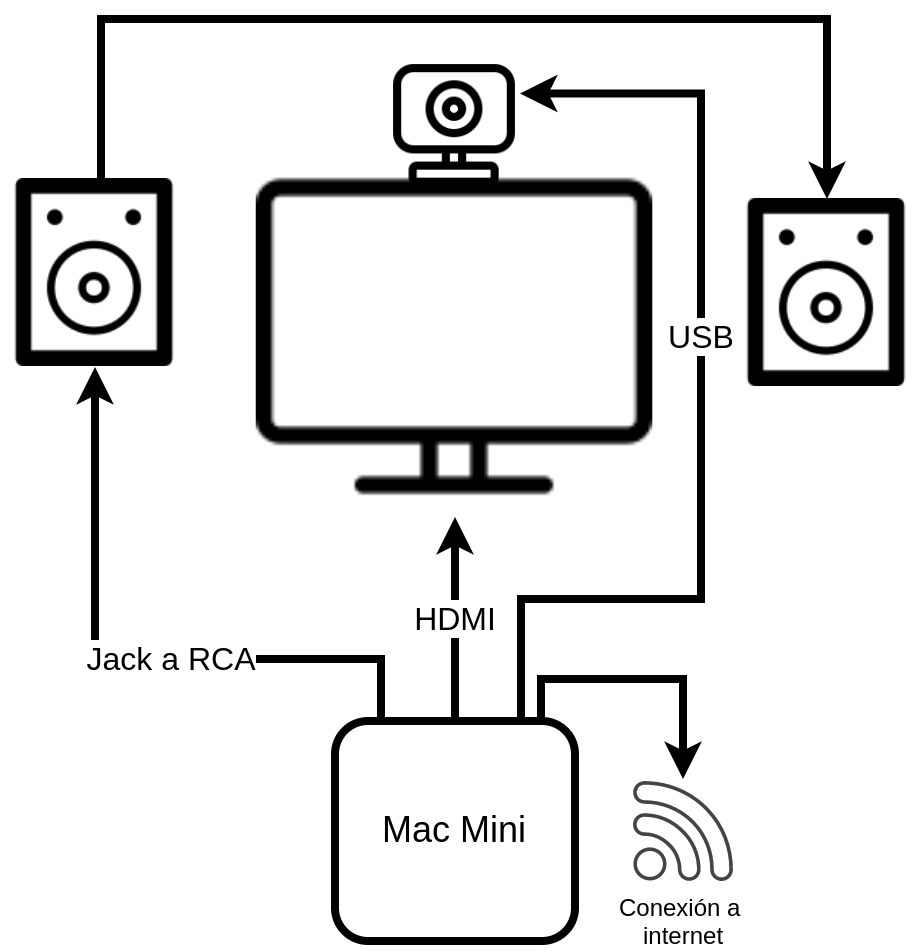
\includegraphics[width=0.7\columnwidth]{../img/antiExWhite.png} 
\caption[Diagrama de Montaje Anti]{Diagrama de montaje de Anti.} % The text in the square bracket is the caption for the list of figures while the text in the curly brackets is the figure caption
\label{fig:gallery} 
\end{figure}

\begin{figure}[tb]
\centering 
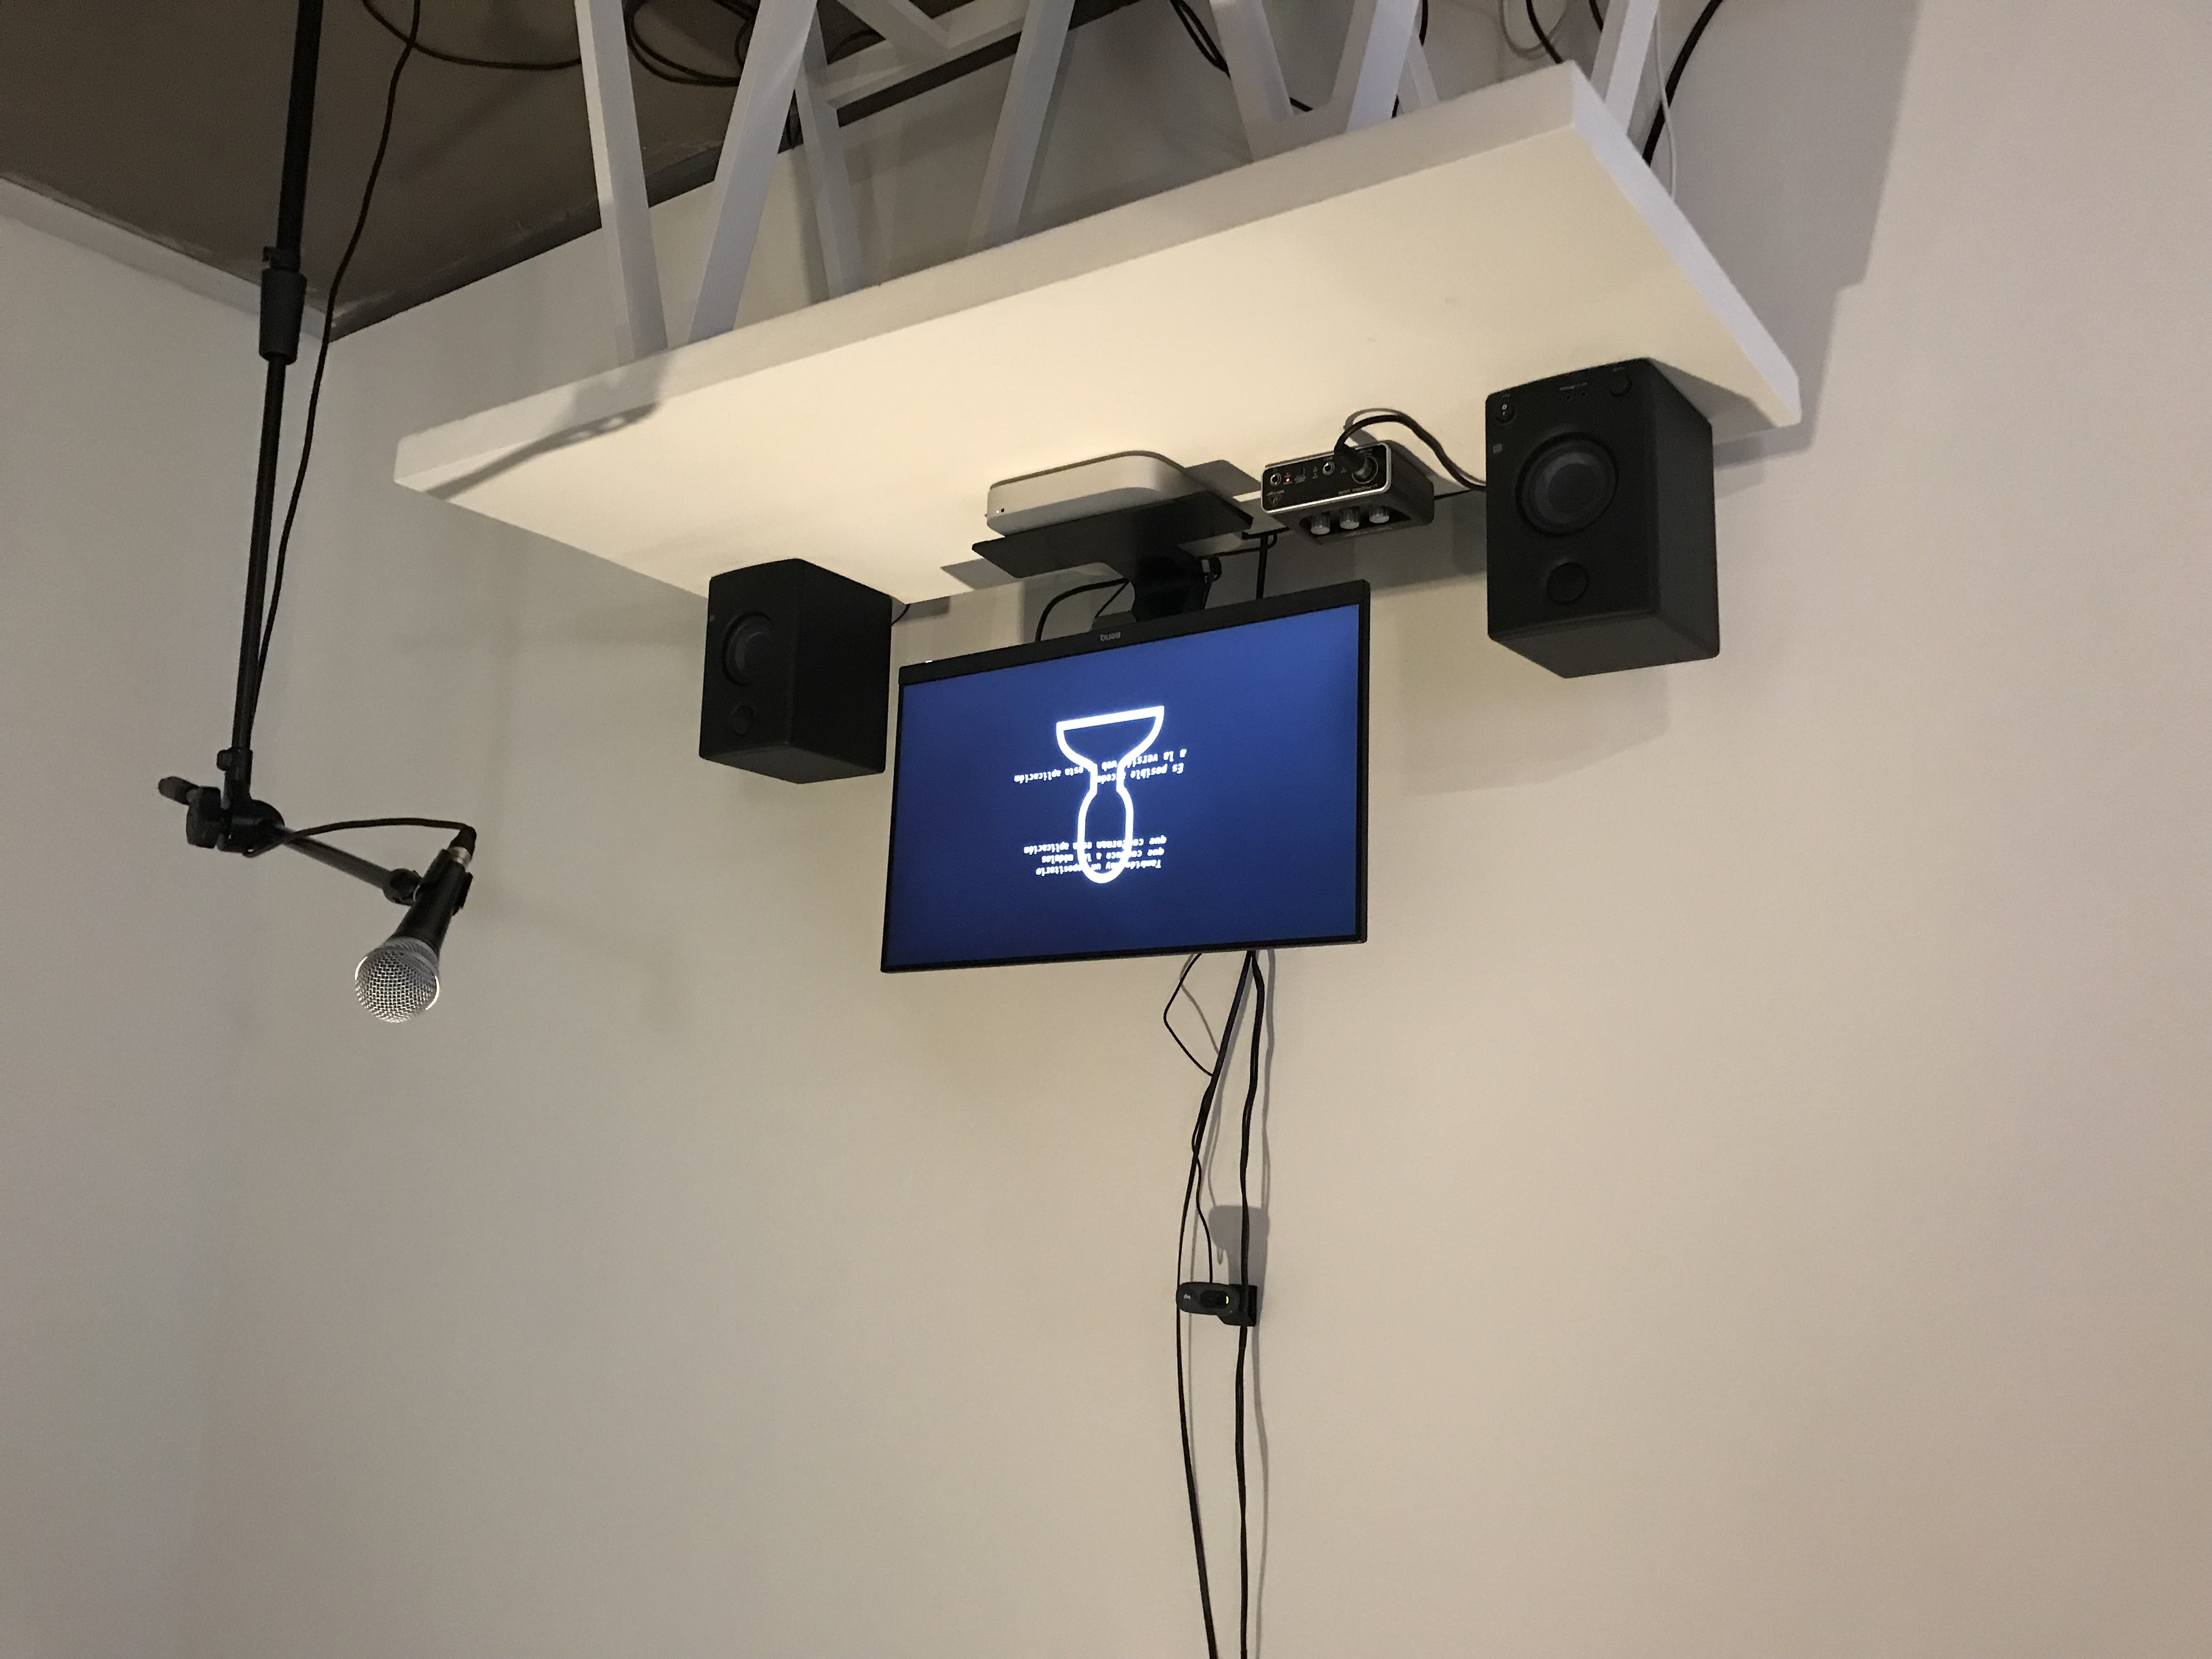
\includegraphics[width=\columnwidth]{../img/ildefonso.jpg} 
\caption[Montaje Anti en San Ildefonso]{Montaje final en el Antiguo Colegio de San Ildefonso} % The text in the square bracket is the caption for the list of figures while the text in the curly brackets is the figure caption
\label{fig:gallery} 
\end{figure}


\subsection{Ecosistema}

Documentación de las piezas que compartieron tiempo y espacio con anti. Preocupaciones compartidas por las consecuencias sociales de la tecnología y el uso responsable de éstas para transformarla, de acuerdo a lo que se mencionó anteriormente de Soon y Cox. Contexto de la desapariciones de los feminicidios en México, la contaminación provocada por el consumo de fast fashion y la relación / interpretación de la realidad a partir de narrativas que contemplan la agencia no-humana. 

La centralidad del individuo 

La idea de múltiples programas de los objetos tecnológicos \citep{latour}

%\section{Descripción técnica general}

Precisión 

\section{Audio e Imagen} % Relevante o puede ir en otro apartado? 

El uso de motores gráficos y de audio decidió el rumbo de la aplicación. Hasta el momento hay dos versiones del proyecto:

\begin{enumerate}

\item La primera versión inicializó el trabajo con recursividad y ejecución de audio por medio de secuenciadores sencillos escritos en Tone.js
\item La segunda versión incorporó a Hydra como una librería externa para la renderización de texturas que pudieran adecuarse a las posibilidades de ofuscación de la capa que \emph{complejizaba} la lectura del rostro
\item Tentativamente la tercera versión se desplazará del entorno de renderización Hydra para explorar las posibilidades de la generación de texturas por medio de shaders.
  
\end{enumerate}

\subsection{Audio}

¿Por qué Tone.js? 

\subsection{Imagen}

¿Por qué Three.js?
keypoints y la construcción de meshes > triangulaciones y las convenciones del modelado tridimensional 

Hydra como un módulo para generar texturas en sólidos 

%\subsection{Redirección de flujos de audio y sonido}

\section{Eventos}

\subsection{Puntos y desarrollo}

El desplazamiento del evento musical y la diversificación de los materiales. Peculiaridades del texto, sonido e imagen. Eventos que establecen puntos de salida y de llegada. Preguntas sobre lo que existe entre puntos. La rampa de tiempo como una forma de relacionar eventualidades y desarrollarlas en el tiempo.

\subsection{Transducción de magnitudes}

Relaciones y diferencias. Transducción de magnitudes 

La biblioteca MediaPipe Facemesh devuelve 468 puntos de referencia faciales. ¿Cómo estos puntos son relevantes? 

Promedios de movimiento asociados a todo y a regiones del rostro. 

\subsection{Materiales}

%\subsection{Materiales y organización}

En esta parte se distribuyeron los materiales sonoros, visuales y textuales en eventos que pudieran detonarse a partir de un esquema temporal y espacial a manera de partitura. 

Texturas

\section{El tiempo en el navegador}

\subsection{Tiempo y secuenciación}

Este apartado puede hablar de las diferencias que existen entre las distintas formas de transformar eventos en el tiempo: setInterval, requestAnimationFrame, Tweenjs y los objetos de Tone.js que permiten detonar eventos como si fueran secuenciadores. Hasta el momento se han detectado tres tipos de aproximaciones: 1) Aquella que está medida en microsegundos y que no necesariamente es precisa, 2) aquella que tiene que ver con temporalidades medidas en segundos ( de hecho el diseño de la estructura general de la pieza tomó esta división con punto de partida y 3) la aproximación que coincide con la convención musical basada en golpes por segundo (BPM). 

\subsection{Panorámica}

Partitura

\begin{figure}[tb]
\centering 
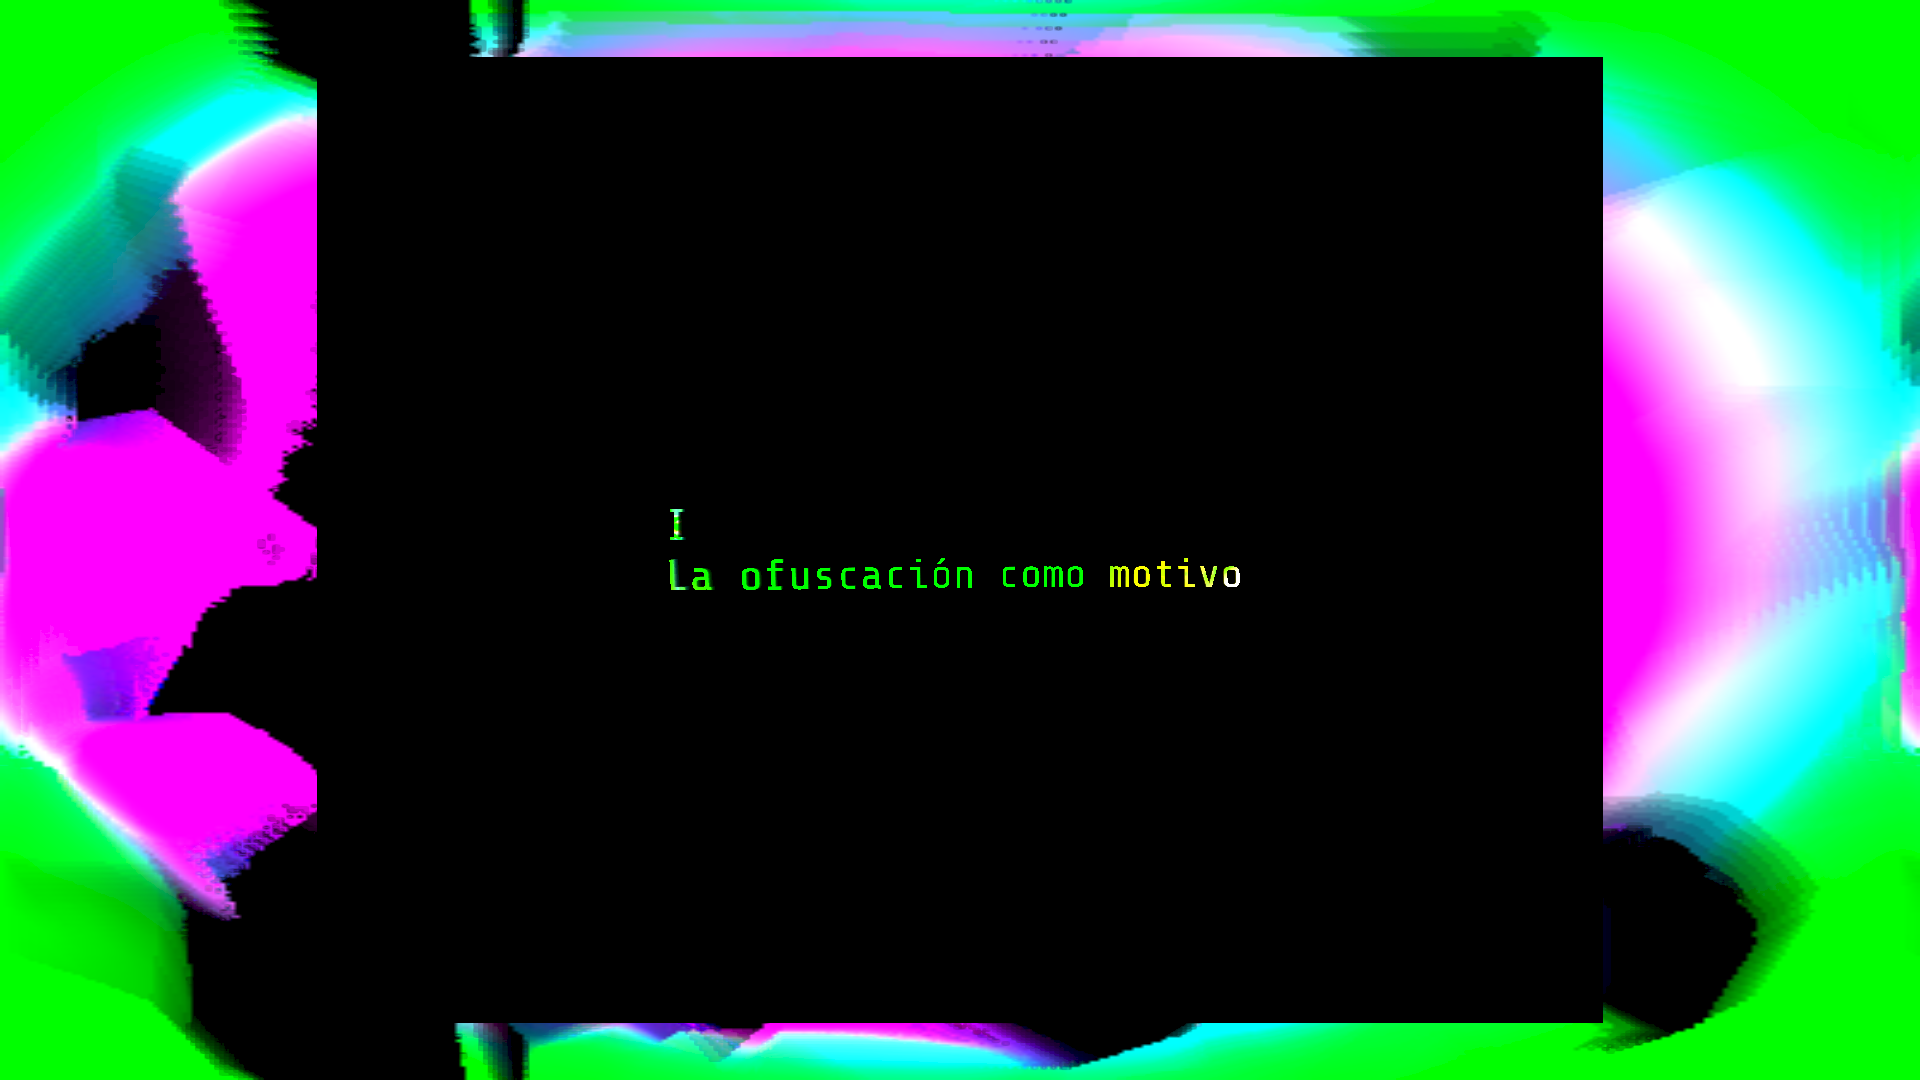
\includegraphics[width=\columnwidth]{../img/antiHydra1.png} 
\caption[Título 1]{Primer título de anti}
\label{fig:gallery} 
\end{figure}

\section{La ofuscación como motivo}

\subsection{Predicciones}

Anti utiliza la biblioteca MediaPipe Facemesh\footnote{MediaPipe Facemesh un un paquete ligero que predice 486 puntos faciales tridimensionales para inferir la superficie geométrica aproximada de una cara humana. Consultado el \today en: Nota: esperar a que suban el paquete} para la detección de puntos de referencia faciales. Estos puntos están optimizados para que las zonas de la cara con mayor gestualidad tengan una densidad de puntos mayor. \citep{kartynnik2019realtime}.

\subsection{Ofuscación audiovisual}

Aquí podría hablar de los aspectos tecnológicos que motivaron la realización de la pieza. Tecnologías diversas que pueden coincidir (no necesariamente lo hacen, por lo menosen términos de la declaratoria y motivación de los proyectos) con la ofuscación facial. Tensorflow y face-landmark-detection. 
te

\begin{figure}[tb]
\centering 
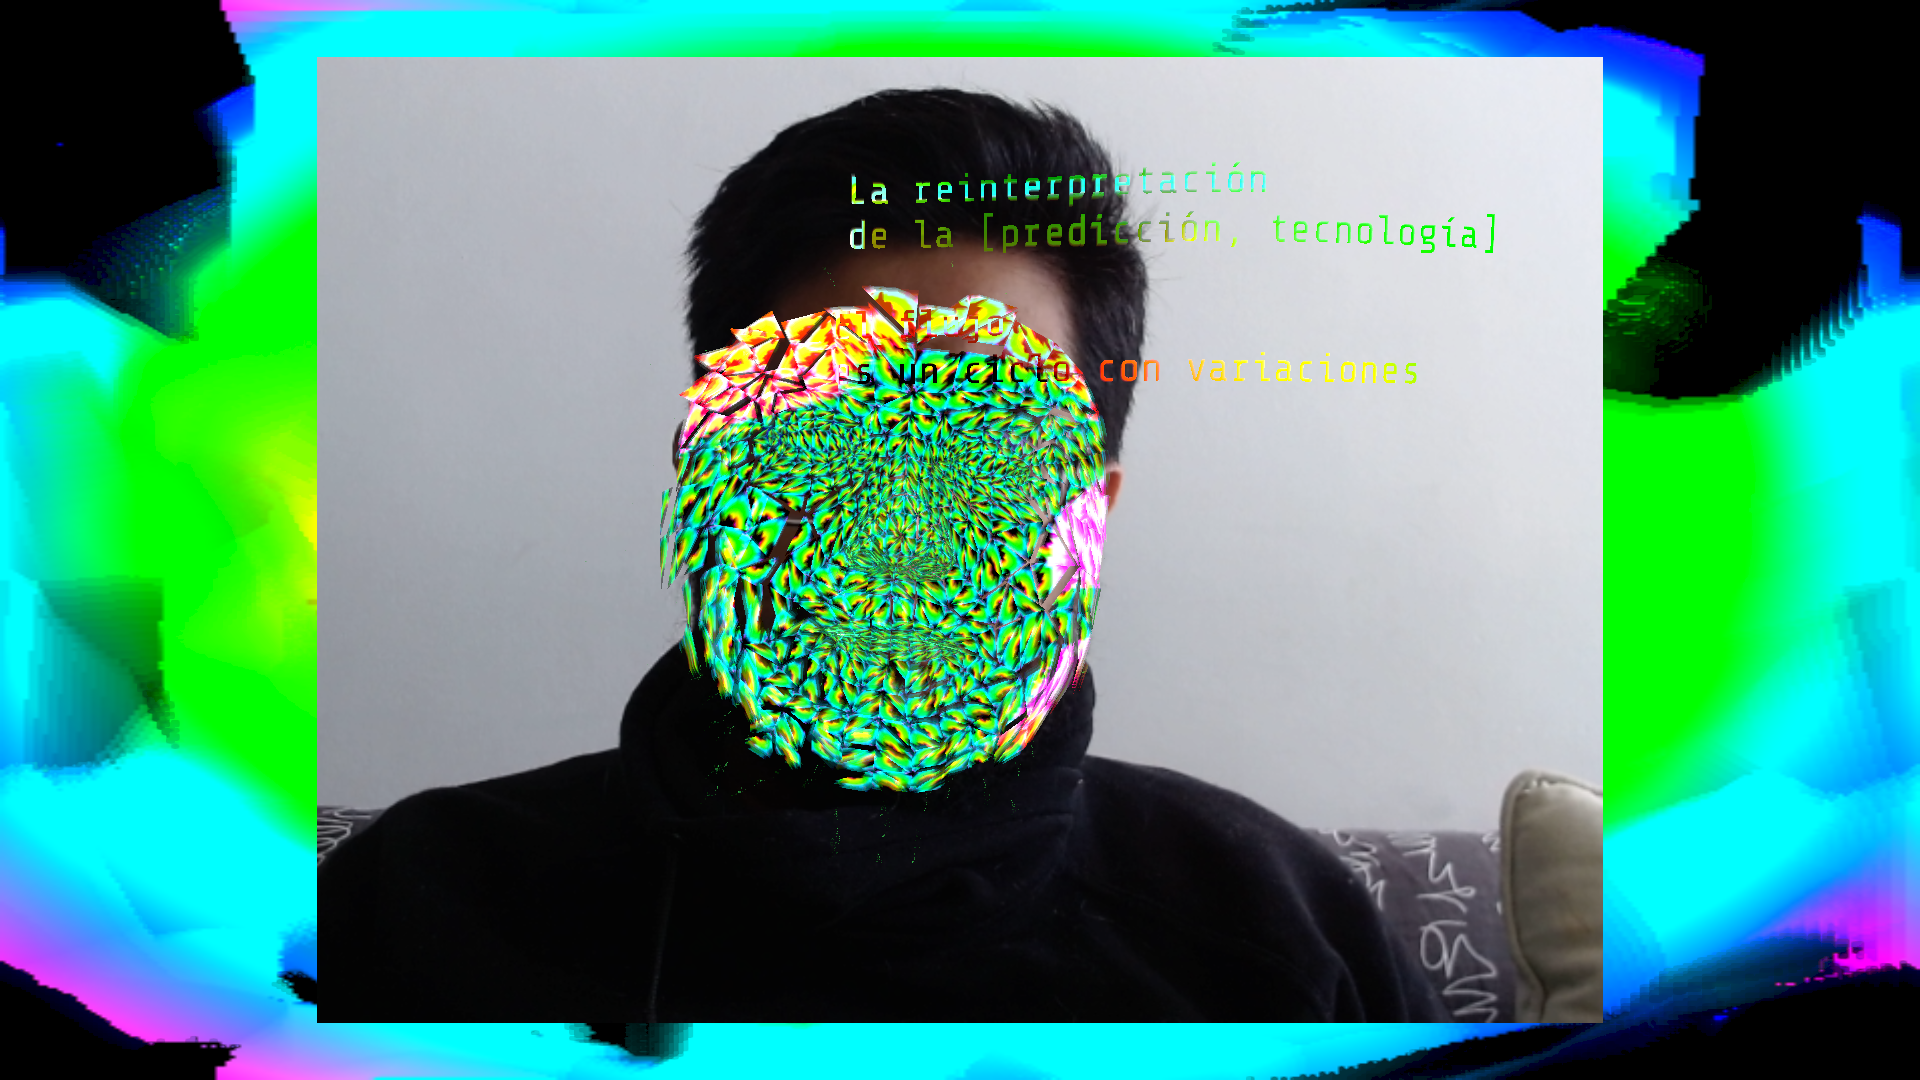
\includegraphics[width=\columnwidth]{../img/antiHydra2.png} 
\caption[Captura Segunda Versión Anti]{Captura de la segunda versión de Anti}
\label{fig:gallery} 
\end{figure}

\subsection{Mediciones}

Plantear la posibilidad de medir el éxito del proyecto con algoritmos de reconocimiento facial. Dar la vuelta a la tecnología como ofuscación y como posibilidad de éxito frente a esa ofuscación. Mediación del diseño humano, decisiones subjetivas basadas en la experiencia. 

Desde el punto de vista humano ¿existe una retroalimentación adversarial que por un lado alimenta la base de datos que un sistema una computadora utiliza y que como parte de un continuo que no se interrumpe, se alimenta y se ve cuestionado / reforzado en cada iteración? ¿

\section{La escritura como rodeo} % Otra palabra que no sea rodeo 

Resultados y giros. 
Distinción entre investigación / práctica artística y manifiesto 
Escritura de código.

% Texto académico vs && || manifiesto 

Desplazamiento del sonido 

%\subsection{Planteamiento Inicial}
%\subsection{Proceso y realización}
%\subsection{Resultados}

%\chapter{Retro}

La recursividad como un motivo presente en las artes electrónicas. ¿Es posible pensar qu hay una retroalimentación no solamente en el dominio técnico, sino tambien en el planteamiento de un flujo interpretativo que el ciertas circustancias se puede acotar a la definición de sintáxis personalizadas para la resulución de un objetivo? me imagino que la respuesta puede conducir a ejemplos delimitados y actuales. 

Recursividad 

Holaaa


%\chapter{Retro}

La recursividad como un motivo presente en las artes electrónicas. ¿Es posible pensar qu hay una retroalimentación no solamente en el dominio técnico, sino tambien en el planteamiento de un flujo interpretativo que el ciertas circustancias se puede acotar a la definición de sintáxis personalizadas para la resulución de un objetivo? me imagino que la respuesta puede conducir a ejemplos delimitados y actuales. 

Recursividad 

Holaaa

% Segundo capítulo 


% Tercer capítulo 

% \chapter{Escritura}


% \chapter{Conclusiones}

% Qué papel tienen las "ciencias del espíritu" de cara a la investigación artística que se centra en un tivo de investigación de las "ciencias exactas / naturales" ? 


\addcontentsline{toc}{chapter}{\protect\numberline{}Referencias}%
\bibliography{../bib/panBib}{} 
\bibliographystyle{../bib/apalike-es}
\clearpage

%\printglossaries

\end{document}
